\documentclass[twoside]{book}

% Packages required by doxygen
\usepackage{fixltx2e}
\usepackage{calc}
\usepackage{doxygen}
\usepackage[export]{adjustbox} % also loads graphicx
\usepackage{graphicx}
\usepackage[utf8]{inputenc}
\usepackage{makeidx}
\usepackage{multicol}
\usepackage{multirow}
\PassOptionsToPackage{warn}{textcomp}
\usepackage{textcomp}
\usepackage[nointegrals]{wasysym}
\usepackage[table]{xcolor}

% Font selection
\usepackage[T1]{fontenc}
\usepackage[scaled=.90]{helvet}
\usepackage{courier}
\usepackage{amssymb}
\usepackage{sectsty}
\renewcommand{\familydefault}{\sfdefault}
\allsectionsfont{%
  \fontseries{bc}\selectfont%
  \color{darkgray}%
}
\renewcommand{\DoxyLabelFont}{%
  \fontseries{bc}\selectfont%
  \color{darkgray}%
}
\newcommand{\+}{\discretionary{\mbox{\scriptsize$\hookleftarrow$}}{}{}}

% Page & text layout
\usepackage{geometry}
\geometry{%
  a4paper,%
  top=2.5cm,%
  bottom=2.5cm,%
  left=2.5cm,%
  right=2.5cm%
}
\tolerance=750
\hfuzz=15pt
\hbadness=750
\setlength{\emergencystretch}{15pt}
\setlength{\parindent}{0cm}
\setlength{\parskip}{3ex plus 2ex minus 2ex}
\makeatletter
\renewcommand{\paragraph}{%
  \@startsection{paragraph}{4}{0ex}{-1.0ex}{1.0ex}{%
    \normalfont\normalsize\bfseries\SS@parafont%
  }%
}
\renewcommand{\subparagraph}{%
  \@startsection{subparagraph}{5}{0ex}{-1.0ex}{1.0ex}{%
    \normalfont\normalsize\bfseries\SS@subparafont%
  }%
}
\makeatother

% Headers & footers
\usepackage{fancyhdr}
\pagestyle{fancyplain}
\fancyhead[LE]{\fancyplain{}{\bfseries\thepage}}
\fancyhead[CE]{\fancyplain{}{}}
\fancyhead[RE]{\fancyplain{}{\bfseries\leftmark}}
\fancyhead[LO]{\fancyplain{}{\bfseries\rightmark}}
\fancyhead[CO]{\fancyplain{}{}}
\fancyhead[RO]{\fancyplain{}{\bfseries\thepage}}
\fancyfoot[LE]{\fancyplain{}{}}
\fancyfoot[CE]{\fancyplain{}{}}
\fancyfoot[RE]{\fancyplain{}{\bfseries\scriptsize Generated by Doxygen }}
\fancyfoot[LO]{\fancyplain{}{\bfseries\scriptsize Generated by Doxygen }}
\fancyfoot[CO]{\fancyplain{}{}}
\fancyfoot[RO]{\fancyplain{}{}}
\renewcommand{\footrulewidth}{0.4pt}
\renewcommand{\chaptermark}[1]{%
  \markboth{#1}{}%
}
\renewcommand{\sectionmark}[1]{%
  \markright{\thesection\ #1}%
}

% Indices & bibliography
\usepackage{natbib}
\usepackage[titles]{tocloft}
\setcounter{tocdepth}{3}
\setcounter{secnumdepth}{5}
\makeindex

% Hyperlinks (required, but should be loaded last)
\usepackage{ifpdf}
\ifpdf
  \usepackage[pdftex,pagebackref=true]{hyperref}
\else
  \usepackage[ps2pdf,pagebackref=true]{hyperref}
\fi
\hypersetup{%
  colorlinks=true,%
  linkcolor=blue,%
  citecolor=blue,%
  unicode%
}

% Custom commands
\newcommand{\clearemptydoublepage}{%
  \newpage{\pagestyle{empty}\cleardoublepage}%
}

\usepackage{caption}
\captionsetup{labelsep=space,justification=centering,font={bf},singlelinecheck=off,skip=4pt,position=top}

%===== C O N T E N T S =====

\begin{document}

% Titlepage & ToC
\hypersetup{pageanchor=false,
             bookmarksnumbered=true,
             pdfencoding=unicode
            }
\pagenumbering{roman}
\begin{titlepage}
\vspace*{7cm}
\begin{center}%
{\Large My Project }\\
\vspace*{1cm}
{\large Generated by Doxygen 1.8.11}\\
\end{center}
\end{titlepage}
\clearemptydoublepage
\tableofcontents
\clearemptydoublepage
\pagenumbering{arabic}
\hypersetup{pageanchor=true}

%--- Begin generated contents ---
\chapter{Namespace Index}
\section{Namespace List}
Here is a list of all documented namespaces with brief descriptions\+:\begin{DoxyCompactList}
\item\contentsline{section}{\hyperlink{namespacegraph}{graph} \\*Graph namespace }{\pageref{namespacegraph}}{}
\end{DoxyCompactList}

\chapter{Hierarchical Index}
\section{Class Hierarchy}
This inheritance list is sorted roughly, but not completely, alphabetically\+:\begin{DoxyCompactList}
\item \contentsline{section}{edge}{\pageref{structedge}}{}
\item \contentsline{section}{Input}{\pageref{classInput}}{}
\item \contentsline{section}{Output}{\pageref{classOutput}}{}
\begin{DoxyCompactList}
\item \contentsline{section}{Interactive\+\_\+editor}{\pageref{classInteractive__editor}}{}
\end{DoxyCompactList}
\item \contentsline{section}{plane}{\pageref{structplane}}{}
\item \contentsline{section}{point}{\pageref{structpoint}}{}
\item \contentsline{section}{Three\+D\+Graph\+\_\+class}{\pageref{classThreeDGraph__class}}{}
\item \contentsline{section}{Two\+D\+Graph\+\_\+class}{\pageref{classTwoDGraph__class}}{}
\end{DoxyCompactList}

\chapter{Class Index}
\section{Class List}
Here are the classes, structs, unions and interfaces with brief descriptions\+:\begin{DoxyCompactList}
\item\contentsline{section}{\hyperlink{classInput}{Input} \\*\hyperlink{classInput}{Input} class }{\pageref{classInput}}{}
\item\contentsline{section}{\hyperlink{classOutput}{Output} \\*Render and save class }{\pageref{classOutput}}{}
\item\contentsline{section}{\hyperlink{classThreeDGraph}{Three\+D\+Graph} \\*3D behaviour class }{\pageref{classThreeDGraph}}{}
\item\contentsline{section}{\hyperlink{classTwoDGraph}{Two\+D\+Graph} \\*2D behaviour class }{\pageref{classTwoDGraph}}{}
\end{DoxyCompactList}

\chapter{File Index}
\section{File List}
Here is a list of all documented files with brief descriptions\+:\begin{DoxyCompactList}
\item\contentsline{section}{Include/\hyperlink{2DProcessingSrc_8h}{2\+D\+Processing\+Src.\+h} }{\pageref{2DProcessingSrc_8h}}{}
\item\contentsline{section}{Include/\hyperlink{3DProcessingSrc_8h}{3\+D\+Processing\+Src.\+h} }{\pageref{3DProcessingSrc_8h}}{}
\item\contentsline{section}{Include/\hyperlink{InputSrc_8h}{Input\+Src.\+h} }{\pageref{InputSrc_8h}}{}
\item\contentsline{section}{Include/\hyperlink{InteractiveSrc_8h}{Interactive\+Src.\+h} }{\pageref{InteractiveSrc_8h}}{}
\item\contentsline{section}{Include/\hyperlink{OutputSrc_8h}{Output\+Src.\+h} }{\pageref{OutputSrc_8h}}{}
\item\contentsline{section}{Include/\hyperlink{structs_8h}{structs.\+h} }{\pageref{structs_8h}}{}
\item\contentsline{section}{Src/\hyperlink{2DProcessingSrc_8cpp}{2\+D\+Processing\+Src.\+cpp} }{\pageref{2DProcessingSrc_8cpp}}{}
\item\contentsline{section}{Src/\hyperlink{3DProcessingSrc_8cpp}{3\+D\+Processing\+Src.\+cpp} }{\pageref{3DProcessingSrc_8cpp}}{}
\item\contentsline{section}{Src/\hyperlink{Index_8cpp}{Index.\+cpp} }{\pageref{Index_8cpp}}{}
\item\contentsline{section}{Src/\hyperlink{IndexTerminal_8cpp}{Index\+Terminal.\+cpp} }{\pageref{IndexTerminal_8cpp}}{}
\item\contentsline{section}{Src/\hyperlink{InputSrc_8cpp}{Input\+Src.\+cpp} }{\pageref{InputSrc_8cpp}}{}
\item\contentsline{section}{Src/\hyperlink{InteractiveSrc_8cpp}{Interactive\+Src.\+cpp} }{\pageref{InteractiveSrc_8cpp}}{}
\item\contentsline{section}{Src/\hyperlink{OutputSrc_8cpp}{Output\+Src.\+cpp} }{\pageref{OutputSrc_8cpp}}{}
\item\contentsline{section}{Src/\hyperlink{structs_8cpp}{structs.\+cpp} }{\pageref{structs_8cpp}}{}
\end{DoxyCompactList}

\chapter{Namespace Documentation}
\hypertarget{namespacegraph}{}\section{graph Namespace Reference}
\label{namespacegraph}\index{graph@{graph}}


Graph namespace.  


\subsection*{Variables}
\begin{DoxyCompactItemize}
\item 
string \hyperlink{namespacegraph_ae7ef3a07e00c4b673fc5d6254cf20f34}{Three\+Dgraph}
\item 
string \hyperlink{namespacegraph_a718228685c9255e4d36f3f3c1294e607}{Two\+Dgraphs} \mbox{[}3\mbox{]}
\item 
boolean \hyperlink{namespacegraph_ae9531d9ba52931cf97c3423d61ba8e5d}{Three\+D\+Or\+TwoD} = false
\end{DoxyCompactItemize}


\subsection{Detailed Description}
Graph namespace. 

This namespace contains the graphs which will be accessed by all the other classes to edit 

\subsection{Variable Documentation}
\index{graph@{graph}!Three\+Dgraph@{Three\+Dgraph}}
\index{Three\+Dgraph@{Three\+Dgraph}!graph@{graph}}
\subsubsection[{\texorpdfstring{Three\+Dgraph}{ThreeDgraph}}]{\setlength{\rightskip}{0pt plus 5cm}string graph\+::\+Three\+Dgraph}\hypertarget{namespacegraph_ae7ef3a07e00c4b673fc5d6254cf20f34}{}\label{namespacegraph_ae7ef3a07e00c4b673fc5d6254cf20f34}
This is the filename \index{graph@{graph}!Three\+D\+Or\+TwoD@{Three\+D\+Or\+TwoD}}
\index{Three\+D\+Or\+TwoD@{Three\+D\+Or\+TwoD}!graph@{graph}}
\subsubsection[{\texorpdfstring{Three\+D\+Or\+TwoD}{ThreeDOrTwoD}}]{\setlength{\rightskip}{0pt plus 5cm}boolean graph\+::\+Three\+D\+Or\+TwoD = false}\hypertarget{namespacegraph_ae9531d9ba52931cf97c3423d61ba8e5d}{}\label{namespacegraph_ae9531d9ba52931cf97c3423d61ba8e5d}
This is flag for checking whether 3d graph is worked upon or 2D graph. True implies 3D graph \index{graph@{graph}!Two\+Dgraphs@{Two\+Dgraphs}}
\index{Two\+Dgraphs@{Two\+Dgraphs}!graph@{graph}}
\subsubsection[{\texorpdfstring{Two\+Dgraphs}{TwoDgraphs}}]{\setlength{\rightskip}{0pt plus 5cm}string graph\+::\+Two\+Dgraphs\mbox{[}3\mbox{]}}\hypertarget{namespacegraph_a718228685c9255e4d36f3f3c1294e607}{}\label{namespacegraph_a718228685c9255e4d36f3f3c1294e607}
This is flag for checking interactive input or file input from the user 
\chapter{Class Documentation}
\hypertarget{structedge}{}\section{edge Struct Reference}
\label{structedge}\index{edge@{edge}}


Struct edge.  




Collaboration diagram for edge\+:
\nopagebreak
\begin{figure}[H]
\begin{center}
\leavevmode
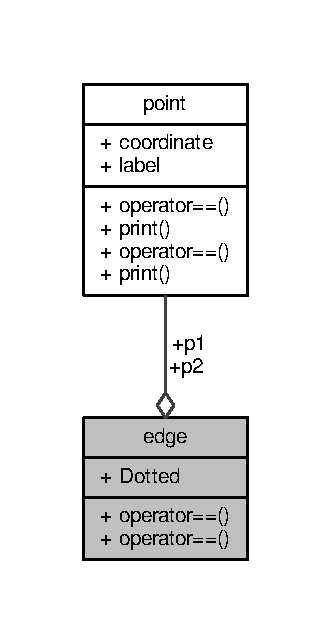
\includegraphics[width=174pt]{structedge__coll__graph}
\end{center}
\end{figure}
\subsection*{Public Attributes}
\begin{DoxyCompactItemize}
\item 
\hyperlink{structpoint}{point} {\bfseries p1}\hypertarget{structedge_a7b074374ee3059d29a93e9e76480274e}{}\label{structedge_a7b074374ee3059d29a93e9e76480274e}

\item 
\hyperlink{structpoint}{point} {\bfseries p2}\hypertarget{structedge_a105ba74e7b01aba7e0e113ab286dc883}{}\label{structedge_a105ba74e7b01aba7e0e113ab286dc883}

\end{DoxyCompactItemize}


\subsection{Detailed Description}
Struct edge. 

This struct represents an edge, as we know two points uniquely determine a line. 

The documentation for this struct was generated from the following file\+:\begin{DoxyCompactItemize}
\item 
\hyperlink{structs_8cpp}{structs.\+cpp}\end{DoxyCompactItemize}

\hypertarget{classInput}{}\section{Input Class Reference}
\label{classInput}\index{Input@{Input}}


\hyperlink{classInput}{Input} class.  




{\ttfamily \#include $<$Input\+Src.\+h$>$}

\subsection*{Public Member Functions}
\begin{DoxyCompactItemize}
\item 
void \hyperlink{classInput_a45065353b80f9980111402e827aae0fe}{get\+File\+Name} (string \hyperlink{classInput_ad073fa115ead2e8b7492214215ebd22d}{file}, bool threeD)
\item 
void \hyperlink{classInput_a9d9395f68b01faa00f962791878723a2}{Read\+File} ()
\item 
void {\bfseries print} ()\hypertarget{classInput_a862e529a6ed3fcfd0719274a04174b7d}{}\label{classInput_a862e529a6ed3fcfd0719274a04174b7d}

\item 
void {\bfseries print3D} ()\hypertarget{classInput_aced126e54ffa271b2a40f7e7a5e90376}{}\label{classInput_aced126e54ffa271b2a40f7e7a5e90376}

\end{DoxyCompactItemize}
\subsection*{Public Attributes}
\begin{DoxyCompactItemize}
\item 
string \hyperlink{classInput_af296359065236ac9139aab7736d6844d}{filename}
\item 
bool \hyperlink{classInput_ad073fa115ead2e8b7492214215ebd22d}{file} = false
\item 
bool \hyperlink{classInput_aacb0e034125e32179081a97eecab47df}{Three\+Dfile} = false
\item 
int \hyperlink{classInput_a82141fe9142aec447f9ef52fd2f78c73}{Two\+D\+File\+Count} = 0
\item 
map$<$ string, vector$<$ \hyperlink{structpoint}{point} $>$ $>$ \hyperlink{classInput_a55526617adbcb0db4b3d565f4dbe772d}{Two\+D\+Graph} \mbox{[}3\mbox{]}
\item 
map$<$ string, vector$<$ \hyperlink{structpoint}{point} $>$ $>$ \hyperlink{classInput_aed882deebbb45d8423e5477e8ccaee60}{Three\+D\+Graph}
\end{DoxyCompactItemize}


\subsection{Detailed Description}
\hyperlink{classInput}{Input} class. 

This class contains the methods to input content from a file or drawing etc.. 

\subsection{Member Function Documentation}
\index{Input@{Input}!get\+File\+Name@{get\+File\+Name}}
\index{get\+File\+Name@{get\+File\+Name}!Input@{Input}}
\subsubsection[{\texorpdfstring{get\+File\+Name(string file, bool three\+D)}{getFileName(string file, bool threeD)}}]{\setlength{\rightskip}{0pt plus 5cm}void Input\+::get\+File\+Name (
\begin{DoxyParamCaption}
\item[{string}]{file, }
\item[{bool}]{threeD}
\end{DoxyParamCaption}
)}\hypertarget{classInput_a45065353b80f9980111402e827aae0fe}{}\label{classInput_a45065353b80f9980111402e827aae0fe}
Will prompt the user for filename or through G\+UI \index{Input@{Input}!Read\+File@{Read\+File}}
\index{Read\+File@{Read\+File}!Input@{Input}}
\subsubsection[{\texorpdfstring{Read\+File()}{ReadFile()}}]{\setlength{\rightskip}{0pt plus 5cm}void Input\+::\+Read\+File (
\begin{DoxyParamCaption}
{}
\end{DoxyParamCaption}
)}\hypertarget{classInput_a9d9395f68b01faa00f962791878723a2}{}\label{classInput_a9d9395f68b01faa00f962791878723a2}

\begin{DoxyParams}{Parameters}
{\em filename} & a string argument. \\
\hline
{\em Three\+Dor\+TwoD} & boolean character to tell the type of file (3\+D/2D). \\
\hline
\end{DoxyParams}


\subsection{Member Data Documentation}
\index{Input@{Input}!file@{file}}
\index{file@{file}!Input@{Input}}
\subsubsection[{\texorpdfstring{file}{file}}]{\setlength{\rightskip}{0pt plus 5cm}bool Input\+::file = false}\hypertarget{classInput_ad073fa115ead2e8b7492214215ebd22d}{}\label{classInput_ad073fa115ead2e8b7492214215ebd22d}
This is flag for checking interactive input or file input from the user \index{Input@{Input}!filename@{filename}}
\index{filename@{filename}!Input@{Input}}
\subsubsection[{\texorpdfstring{filename}{filename}}]{\setlength{\rightskip}{0pt plus 5cm}string Input\+::filename}\hypertarget{classInput_af296359065236ac9139aab7736d6844d}{}\label{classInput_af296359065236ac9139aab7736d6844d}
This is the filename \index{Input@{Input}!Three\+Dfile@{Three\+Dfile}}
\index{Three\+Dfile@{Three\+Dfile}!Input@{Input}}
\subsubsection[{\texorpdfstring{Three\+Dfile}{ThreeDfile}}]{\setlength{\rightskip}{0pt plus 5cm}bool Input\+::\+Three\+Dfile = false}\hypertarget{classInput_aacb0e034125e32179081a97eecab47df}{}\label{classInput_aacb0e034125e32179081a97eecab47df}
This is flag for checking whether file has 3D or 2D input \index{Input@{Input}!Three\+D\+Graph@{Three\+D\+Graph}}
\index{Three\+D\+Graph@{Three\+D\+Graph}!Input@{Input}}
\subsubsection[{\texorpdfstring{Three\+D\+Graph}{ThreeDGraph}}]{\setlength{\rightskip}{0pt plus 5cm}map$<$string, vector$<${\bf point}$>$ $>$ Input\+::\+Three\+D\+Graph}\hypertarget{classInput_aed882deebbb45d8423e5477e8ccaee60}{}\label{classInput_aed882deebbb45d8423e5477e8ccaee60}
This is the 3D graph \index{Input@{Input}!Two\+D\+File\+Count@{Two\+D\+File\+Count}}
\index{Two\+D\+File\+Count@{Two\+D\+File\+Count}!Input@{Input}}
\subsubsection[{\texorpdfstring{Two\+D\+File\+Count}{TwoDFileCount}}]{\setlength{\rightskip}{0pt plus 5cm}int Input\+::\+Two\+D\+File\+Count = 0}\hypertarget{classInput_a82141fe9142aec447f9ef52fd2f78c73}{}\label{classInput_a82141fe9142aec447f9ef52fd2f78c73}
Count of 2D objects as there has to be 3 projections for our software to work on \index{Input@{Input}!Two\+D\+Graph@{Two\+D\+Graph}}
\index{Two\+D\+Graph@{Two\+D\+Graph}!Input@{Input}}
\subsubsection[{\texorpdfstring{Two\+D\+Graph}{TwoDGraph}}]{\setlength{\rightskip}{0pt plus 5cm}map$<$string, vector$<${\bf point}$>$ $>$ Input\+::\+Two\+D\+Graph\mbox{[}3\mbox{]}}\hypertarget{classInput_a55526617adbcb0db4b3d565f4dbe772d}{}\label{classInput_a55526617adbcb0db4b3d565f4dbe772d}
This is the array of orthographic projections 

The documentation for this class was generated from the following files\+:\begin{DoxyCompactItemize}
\item 
\hyperlink{InputSrc_8h}{Input\+Src.\+h}\item 
\hyperlink{InputSrc_8cpp}{Input\+Src.\+cpp}\end{DoxyCompactItemize}

\hypertarget{classInteractive__editor}{}\section{Interactive\+\_\+editor Class Reference}
\label{classInteractive__editor}\index{Interactive\+\_\+editor@{Interactive\+\_\+editor}}


Editor class.  




{\ttfamily \#include $<$Interactive\+Src.\+h$>$}

\subsection*{Public Member Functions}
\begin{DoxyCompactItemize}
\item 
void \hyperlink{classInteractive__editor_aa7d472e169eed213d1fcb874c6f5a6cd}{user\+Input} ()
\item 
void \hyperlink{classInteractive__editor_a8078ec1404bdd80e09320d14d198f628}{display\+Options} ()
\item 
void \hyperlink{classInteractive__editor_a5a7723f6affebd15ae935eb48e91359f}{draw\+Line} (\hyperlink{structpoint}{point} p1, \hyperlink{structpoint}{point} p2)
\item 
void \hyperlink{classInteractive__editor_a678c382483cb0b40d1616c1d28eaf200}{erase\+It} (\hyperlink{structpoint}{point} p1, \hyperlink{structpoint}{point} p2)
\item 
void \hyperlink{classInteractive__editor_aedd168ce9dc711e3756aafa44146cb76}{print} ()
\end{DoxyCompactItemize}
\subsection*{Public Attributes}
\begin{DoxyCompactItemize}
\item 
map$<$ string, vector$<$ \hyperlink{structpoint}{point} $>$ $>$ \hyperlink{classInteractive__editor_a1e77c81fdaf1da82816d476fa431fc34}{My\+Plane}
\item 
bool \hyperlink{classInteractive__editor_a66468db06170aca0dae8e057d98253bd}{exit\+Yes\+No}
\item 
bool \hyperlink{classInteractive__editor_a2e6cd28cc09c6250bb5aa720acfc16a4}{saved}
\item 
bool \hyperlink{classInteractive__editor_a82aa208ba6d10c885699d227d928c82c}{save\+To\+File}
\item 
bool \hyperlink{classInteractive__editor_a7af788147541bfc20163c1c2a8550cbe}{save}
\item 
bool \hyperlink{classInteractive__editor_a93c2f2041e432c8047d51942345cc3f9}{type}
\item 
int \hyperlink{classInteractive__editor_a016e5e8e9a124977ab6048c90980be97}{Two\+D\+File\+Number}
\item 
bool \hyperlink{classInteractive__editor_ace62b483a0866c64212ee0c641445c7a}{drawing}
\item 
bool \hyperlink{classInteractive__editor_aa0de8abac09ce2259252fba6c1958e83}{line\+Draw}
\item 
bool \hyperlink{classInteractive__editor_ac2f2f1dfb6c21585d4ed5ed043e41b25}{erase}
\item 
bool \hyperlink{classInteractive__editor_a1688fc65949d3d4c337b7b4e36986f3c}{extrude\+Yes\+No}
\item 
bool \hyperlink{classInteractive__editor_a9da61abe038ee33f9d15ef4a028dc8ab}{select\+Plane}
\item 
bool \hyperlink{classInteractive__editor_ab0f07759c3ff1bcfe45d0c285abe29b5}{select\+Point}
\item 
bool \hyperlink{classInteractive__editor_a69d697425045525e2aadd2eb956fce24}{select\+Line}
\item 
bool \hyperlink{classInteractive__editor_a13a2206b6c7e86947e85830afb229f36}{Convert2\+Dto3D}
\item 
bool \hyperlink{classInteractive__editor_a83829cee0dd00c90dbb841abde5596a4}{Convert3\+Dto2D}
\item 
bool \hyperlink{classInteractive__editor_a9accc369abf6972993bb5c2ba047542c}{rotate}
\item 
int \hyperlink{classInteractive__editor_a07fe2897bcad8eabf5b98e01a162b2a1}{point1}
\item 
int \hyperlink{classInteractive__editor_af60245cb328db4c6b1ca00f1512dfc75}{point2}
\item 
int \hyperlink{classInteractive__editor_a9b368072fc0a220476d21079b4bcb739}{point3}
\item 
int \hyperlink{classInteractive__editor_a65f9bb481055109e9d52e2a6bc2db58e}{thickness}
\item 
int \hyperlink{classInteractive__editor_a8bb78acdc55bebbe34bc545eb720217c}{color}
\item 
int \hyperlink{classInteractive__editor_aced5ec777fe62fb280f3668a1c59f9b7}{height}
\item 
int \hyperlink{classInteractive__editor_acb67c8393df8fe6f6f938f0609f24050}{centre}
\end{DoxyCompactItemize}


\subsection{Detailed Description}
Editor class. 

This class contains the methods to edit a drawing or to play with a model drawing 

\subsection{Member Function Documentation}
\index{Interactive\+\_\+editor@{Interactive\+\_\+editor}!display\+Options@{display\+Options}}
\index{display\+Options@{display\+Options}!Interactive\+\_\+editor@{Interactive\+\_\+editor}}
\subsubsection[{\texorpdfstring{display\+Options()}{displayOptions()}}]{\setlength{\rightskip}{0pt plus 5cm}void Interactive\+\_\+editor\+::display\+Options (
\begin{DoxyParamCaption}
{}
\end{DoxyParamCaption}
)}\hypertarget{classInteractive__editor_a8078ec1404bdd80e09320d14d198f628}{}\label{classInteractive__editor_a8078ec1404bdd80e09320d14d198f628}
Will display the options/settings user desires \index{Interactive\+\_\+editor@{Interactive\+\_\+editor}!draw\+Line@{draw\+Line}}
\index{draw\+Line@{draw\+Line}!Interactive\+\_\+editor@{Interactive\+\_\+editor}}
\subsubsection[{\texorpdfstring{draw\+Line(point p1, point p2)}{drawLine(point p1, point p2)}}]{\setlength{\rightskip}{0pt plus 5cm}void Interactive\+\_\+editor\+::draw\+Line (
\begin{DoxyParamCaption}
\item[{{\bf point}}]{p1, }
\item[{{\bf point}}]{p2}
\end{DoxyParamCaption}
)}\hypertarget{classInteractive__editor_a5a7723f6affebd15ae935eb48e91359f}{}\label{classInteractive__editor_a5a7723f6affebd15ae935eb48e91359f}
Will set the options/settings user desires 
\begin{DoxyParams}{Parameters}
{\em poin1} & To get 1st point of line. \\
\hline
{\em poin2} & To get 2nd point of line. \\
\hline
{\em thickness} & To get thickness of line. \\
\hline
{\em color} & To get color of the line. \\
\hline
\end{DoxyParams}
\index{Interactive\+\_\+editor@{Interactive\+\_\+editor}!erase\+It@{erase\+It}}
\index{erase\+It@{erase\+It}!Interactive\+\_\+editor@{Interactive\+\_\+editor}}
\subsubsection[{\texorpdfstring{erase\+It(point p1, point p2)}{eraseIt(point p1, point p2)}}]{\setlength{\rightskip}{0pt plus 5cm}void Interactive\+\_\+editor\+::erase\+It (
\begin{DoxyParamCaption}
\item[{{\bf point}}]{p1, }
\item[{{\bf point}}]{p2}
\end{DoxyParamCaption}
)}\hypertarget{classInteractive__editor_a678c382483cb0b40d1616c1d28eaf200}{}\label{classInteractive__editor_a678c382483cb0b40d1616c1d28eaf200}
Will set the options/settings user desires \index{Interactive\+\_\+editor@{Interactive\+\_\+editor}!print@{print}}
\index{print@{print}!Interactive\+\_\+editor@{Interactive\+\_\+editor}}
\subsubsection[{\texorpdfstring{print()}{print()}}]{\setlength{\rightskip}{0pt plus 5cm}void Interactive\+\_\+editor\+::print (
\begin{DoxyParamCaption}
{}
\end{DoxyParamCaption}
)}\hypertarget{classInteractive__editor_aedd168ce9dc711e3756aafa44146cb76}{}\label{classInteractive__editor_aedd168ce9dc711e3756aafa44146cb76}
To print the graph \index{Interactive\+\_\+editor@{Interactive\+\_\+editor}!user\+Input@{user\+Input}}
\index{user\+Input@{user\+Input}!Interactive\+\_\+editor@{Interactive\+\_\+editor}}
\subsubsection[{\texorpdfstring{user\+Input()}{userInput()}}]{\setlength{\rightskip}{0pt plus 5cm}void Interactive\+\_\+editor\+::user\+Input (
\begin{DoxyParamCaption}
{}
\end{DoxyParamCaption}
)}\hypertarget{classInteractive__editor_aa7d472e169eed213d1fcb874c6f5a6cd}{}\label{classInteractive__editor_aa7d472e169eed213d1fcb874c6f5a6cd}
Will set the options/settings user desires 
\begin{DoxyParams}{Parameters}
{\em drawing} & To check if user wants to draw something or want to edit the current drawing. \\
\hline
{\em linedraw} & To check if user wants to draw a line. \\
\hline
{\em circledraw} & To check if user wants to draw a cicle. \\
\hline
{\em erase} & To check if user wants to erase something. \\
\hline
{\em extrude} & To check if user wants to extrude a plane. \\
\hline
{\em flag3\+Dfile} & To check if file is input or an intercative input. \\
\hline
\end{DoxyParams}


\subsection{Member Data Documentation}
\index{Interactive\+\_\+editor@{Interactive\+\_\+editor}!centre@{centre}}
\index{centre@{centre}!Interactive\+\_\+editor@{Interactive\+\_\+editor}}
\subsubsection[{\texorpdfstring{centre}{centre}}]{\setlength{\rightskip}{0pt plus 5cm}int Interactive\+\_\+editor\+::centre}\hypertarget{classInteractive__editor_acb67c8393df8fe6f6f938f0609f24050}{}\label{classInteractive__editor_acb67c8393df8fe6f6f938f0609f24050}
This is the height of extrusion W\+H\+AT IS T\+H\+IS? R\+E\+P\+E\+T\+I\+T\+I\+O\+N3 \index{Interactive\+\_\+editor@{Interactive\+\_\+editor}!color@{color}}
\index{color@{color}!Interactive\+\_\+editor@{Interactive\+\_\+editor}}
\subsubsection[{\texorpdfstring{color}{color}}]{\setlength{\rightskip}{0pt plus 5cm}int Interactive\+\_\+editor\+::color}\hypertarget{classInteractive__editor_a8bb78acdc55bebbe34bc545eb720217c}{}\label{classInteractive__editor_a8bb78acdc55bebbe34bc545eb720217c}
This is the color of the line \index{Interactive\+\_\+editor@{Interactive\+\_\+editor}!Convert2\+Dto3D@{Convert2\+Dto3D}}
\index{Convert2\+Dto3D@{Convert2\+Dto3D}!Interactive\+\_\+editor@{Interactive\+\_\+editor}}
\subsubsection[{\texorpdfstring{Convert2\+Dto3D}{Convert2Dto3D}}]{\setlength{\rightskip}{0pt plus 5cm}bool Interactive\+\_\+editor\+::\+Convert2\+Dto3D}\hypertarget{classInteractive__editor_a13a2206b6c7e86947e85830afb229f36}{}\label{classInteractive__editor_a13a2206b6c7e86947e85830afb229f36}
This flag is set to identify whether user wants to convert 2D to 3D \index{Interactive\+\_\+editor@{Interactive\+\_\+editor}!Convert3\+Dto2D@{Convert3\+Dto2D}}
\index{Convert3\+Dto2D@{Convert3\+Dto2D}!Interactive\+\_\+editor@{Interactive\+\_\+editor}}
\subsubsection[{\texorpdfstring{Convert3\+Dto2D}{Convert3Dto2D}}]{\setlength{\rightskip}{0pt plus 5cm}bool Interactive\+\_\+editor\+::\+Convert3\+Dto2D}\hypertarget{classInteractive__editor_a83829cee0dd00c90dbb841abde5596a4}{}\label{classInteractive__editor_a83829cee0dd00c90dbb841abde5596a4}
This flag is set to identify whether user wants to convert 3D to 2D \index{Interactive\+\_\+editor@{Interactive\+\_\+editor}!drawing@{drawing}}
\index{drawing@{drawing}!Interactive\+\_\+editor@{Interactive\+\_\+editor}}
\subsubsection[{\texorpdfstring{drawing}{drawing}}]{\setlength{\rightskip}{0pt plus 5cm}bool Interactive\+\_\+editor\+::drawing}\hypertarget{classInteractive__editor_ace62b483a0866c64212ee0c641445c7a}{}\label{classInteractive__editor_ace62b483a0866c64212ee0c641445c7a}
This flag is set to identify whether user wants to draw or input a file. By Default it is set to file \index{Interactive\+\_\+editor@{Interactive\+\_\+editor}!erase@{erase}}
\index{erase@{erase}!Interactive\+\_\+editor@{Interactive\+\_\+editor}}
\subsubsection[{\texorpdfstring{erase}{erase}}]{\setlength{\rightskip}{0pt plus 5cm}bool Interactive\+\_\+editor\+::erase}\hypertarget{classInteractive__editor_ac2f2f1dfb6c21585d4ed5ed043e41b25}{}\label{classInteractive__editor_ac2f2f1dfb6c21585d4ed5ed043e41b25}
This flag is set to identify whether user wants to erase something or not \index{Interactive\+\_\+editor@{Interactive\+\_\+editor}!exit\+Yes\+No@{exit\+Yes\+No}}
\index{exit\+Yes\+No@{exit\+Yes\+No}!Interactive\+\_\+editor@{Interactive\+\_\+editor}}
\subsubsection[{\texorpdfstring{exit\+Yes\+No}{exitYesNo}}]{\setlength{\rightskip}{0pt plus 5cm}bool Interactive\+\_\+editor\+::exit\+Yes\+No}\hypertarget{classInteractive__editor_a66468db06170aca0dae8e057d98253bd}{}\label{classInteractive__editor_a66468db06170aca0dae8e057d98253bd}
This flag is set to identify whether user has to exit \index{Interactive\+\_\+editor@{Interactive\+\_\+editor}!extrude\+Yes\+No@{extrude\+Yes\+No}}
\index{extrude\+Yes\+No@{extrude\+Yes\+No}!Interactive\+\_\+editor@{Interactive\+\_\+editor}}
\subsubsection[{\texorpdfstring{extrude\+Yes\+No}{extrudeYesNo}}]{\setlength{\rightskip}{0pt plus 5cm}bool Interactive\+\_\+editor\+::extrude\+Yes\+No}\hypertarget{classInteractive__editor_a1688fc65949d3d4c337b7b4e36986f3c}{}\label{classInteractive__editor_a1688fc65949d3d4c337b7b4e36986f3c}
This flag is set to identify whether user wants to extrude something or not \index{Interactive\+\_\+editor@{Interactive\+\_\+editor}!height@{height}}
\index{height@{height}!Interactive\+\_\+editor@{Interactive\+\_\+editor}}
\subsubsection[{\texorpdfstring{height}{height}}]{\setlength{\rightskip}{0pt plus 5cm}int Interactive\+\_\+editor\+::height}\hypertarget{classInteractive__editor_aced5ec777fe62fb280f3668a1c59f9b7}{}\label{classInteractive__editor_aced5ec777fe62fb280f3668a1c59f9b7}
This is the height of extrusion \index{Interactive\+\_\+editor@{Interactive\+\_\+editor}!line\+Draw@{line\+Draw}}
\index{line\+Draw@{line\+Draw}!Interactive\+\_\+editor@{Interactive\+\_\+editor}}
\subsubsection[{\texorpdfstring{line\+Draw}{lineDraw}}]{\setlength{\rightskip}{0pt plus 5cm}bool Interactive\+\_\+editor\+::line\+Draw}\hypertarget{classInteractive__editor_aa0de8abac09ce2259252fba6c1958e83}{}\label{classInteractive__editor_aa0de8abac09ce2259252fba6c1958e83}
This flag is set to identify whether user wants to draw a line or not \index{Interactive\+\_\+editor@{Interactive\+\_\+editor}!My\+Plane@{My\+Plane}}
\index{My\+Plane@{My\+Plane}!Interactive\+\_\+editor@{Interactive\+\_\+editor}}
\subsubsection[{\texorpdfstring{My\+Plane}{MyPlane}}]{\setlength{\rightskip}{0pt plus 5cm}map$<$string, vector$<${\bf point}$>$ $>$ Interactive\+\_\+editor\+::\+My\+Plane}\hypertarget{classInteractive__editor_a1e77c81fdaf1da82816d476fa431fc34}{}\label{classInteractive__editor_a1e77c81fdaf1da82816d476fa431fc34}
This is a plane \index{Interactive\+\_\+editor@{Interactive\+\_\+editor}!point1@{point1}}
\index{point1@{point1}!Interactive\+\_\+editor@{Interactive\+\_\+editor}}
\subsubsection[{\texorpdfstring{point1}{point1}}]{\setlength{\rightskip}{0pt plus 5cm}int Interactive\+\_\+editor\+::point1}\hypertarget{classInteractive__editor_a07fe2897bcad8eabf5b98e01a162b2a1}{}\label{classInteractive__editor_a07fe2897bcad8eabf5b98e01a162b2a1}
This is a point\textquotesingle{}s location on the coordinates \index{Interactive\+\_\+editor@{Interactive\+\_\+editor}!point2@{point2}}
\index{point2@{point2}!Interactive\+\_\+editor@{Interactive\+\_\+editor}}
\subsubsection[{\texorpdfstring{point2}{point2}}]{\setlength{\rightskip}{0pt plus 5cm}int Interactive\+\_\+editor\+::point2}\hypertarget{classInteractive__editor_af60245cb328db4c6b1ca00f1512dfc75}{}\label{classInteractive__editor_af60245cb328db4c6b1ca00f1512dfc75}
This is a point\textquotesingle{}s location on the coordinates \index{Interactive\+\_\+editor@{Interactive\+\_\+editor}!point3@{point3}}
\index{point3@{point3}!Interactive\+\_\+editor@{Interactive\+\_\+editor}}
\subsubsection[{\texorpdfstring{point3}{point3}}]{\setlength{\rightskip}{0pt plus 5cm}int Interactive\+\_\+editor\+::point3}\hypertarget{classInteractive__editor_a9b368072fc0a220476d21079b4bcb739}{}\label{classInteractive__editor_a9b368072fc0a220476d21079b4bcb739}
This is a point\textquotesingle{}s location on the coordinates \index{Interactive\+\_\+editor@{Interactive\+\_\+editor}!rotate@{rotate}}
\index{rotate@{rotate}!Interactive\+\_\+editor@{Interactive\+\_\+editor}}
\subsubsection[{\texorpdfstring{rotate}{rotate}}]{\setlength{\rightskip}{0pt plus 5cm}bool Interactive\+\_\+editor\+::rotate}\hypertarget{classInteractive__editor_a9accc369abf6972993bb5c2ba047542c}{}\label{classInteractive__editor_a9accc369abf6972993bb5c2ba047542c}
This flag is set to identify whether user wants to rotate a 3D object or not \index{Interactive\+\_\+editor@{Interactive\+\_\+editor}!save@{save}}
\index{save@{save}!Interactive\+\_\+editor@{Interactive\+\_\+editor}}
\subsubsection[{\texorpdfstring{save}{save}}]{\setlength{\rightskip}{0pt plus 5cm}bool Interactive\+\_\+editor\+::save}\hypertarget{classInteractive__editor_a7af788147541bfc20163c1c2a8550cbe}{}\label{classInteractive__editor_a7af788147541bfc20163c1c2a8550cbe}
This flag is set to identify whether user has pressed save button \index{Interactive\+\_\+editor@{Interactive\+\_\+editor}!saved@{saved}}
\index{saved@{saved}!Interactive\+\_\+editor@{Interactive\+\_\+editor}}
\subsubsection[{\texorpdfstring{saved}{saved}}]{\setlength{\rightskip}{0pt plus 5cm}bool Interactive\+\_\+editor\+::saved}\hypertarget{classInteractive__editor_a2e6cd28cc09c6250bb5aa720acfc16a4}{}\label{classInteractive__editor_a2e6cd28cc09c6250bb5aa720acfc16a4}
This flag is set to identify whether user has something left to be saved \index{Interactive\+\_\+editor@{Interactive\+\_\+editor}!save\+To\+File@{save\+To\+File}}
\index{save\+To\+File@{save\+To\+File}!Interactive\+\_\+editor@{Interactive\+\_\+editor}}
\subsubsection[{\texorpdfstring{save\+To\+File}{saveToFile}}]{\setlength{\rightskip}{0pt plus 5cm}bool Interactive\+\_\+editor\+::save\+To\+File}\hypertarget{classInteractive__editor_a82aa208ba6d10c885699d227d928c82c}{}\label{classInteractive__editor_a82aa208ba6d10c885699d227d928c82c}
This flag is set to identify whether user has something to be saved in a file \index{Interactive\+\_\+editor@{Interactive\+\_\+editor}!select\+Line@{select\+Line}}
\index{select\+Line@{select\+Line}!Interactive\+\_\+editor@{Interactive\+\_\+editor}}
\subsubsection[{\texorpdfstring{select\+Line}{selectLine}}]{\setlength{\rightskip}{0pt plus 5cm}bool Interactive\+\_\+editor\+::select\+Line}\hypertarget{classInteractive__editor_a69d697425045525e2aadd2eb956fce24}{}\label{classInteractive__editor_a69d697425045525e2aadd2eb956fce24}
This flag is set to identify whether user wants to select a line or not \index{Interactive\+\_\+editor@{Interactive\+\_\+editor}!select\+Plane@{select\+Plane}}
\index{select\+Plane@{select\+Plane}!Interactive\+\_\+editor@{Interactive\+\_\+editor}}
\subsubsection[{\texorpdfstring{select\+Plane}{selectPlane}}]{\setlength{\rightskip}{0pt plus 5cm}bool Interactive\+\_\+editor\+::select\+Plane}\hypertarget{classInteractive__editor_a9da61abe038ee33f9d15ef4a028dc8ab}{}\label{classInteractive__editor_a9da61abe038ee33f9d15ef4a028dc8ab}
This flag is set to identify whether user wants to select a plane or not \index{Interactive\+\_\+editor@{Interactive\+\_\+editor}!select\+Point@{select\+Point}}
\index{select\+Point@{select\+Point}!Interactive\+\_\+editor@{Interactive\+\_\+editor}}
\subsubsection[{\texorpdfstring{select\+Point}{selectPoint}}]{\setlength{\rightskip}{0pt plus 5cm}bool Interactive\+\_\+editor\+::select\+Point}\hypertarget{classInteractive__editor_ab0f07759c3ff1bcfe45d0c285abe29b5}{}\label{classInteractive__editor_ab0f07759c3ff1bcfe45d0c285abe29b5}
This flag is set to identify whether user wants to select a point or not \index{Interactive\+\_\+editor@{Interactive\+\_\+editor}!thickness@{thickness}}
\index{thickness@{thickness}!Interactive\+\_\+editor@{Interactive\+\_\+editor}}
\subsubsection[{\texorpdfstring{thickness}{thickness}}]{\setlength{\rightskip}{0pt plus 5cm}int Interactive\+\_\+editor\+::thickness}\hypertarget{classInteractive__editor_a65f9bb481055109e9d52e2a6bc2db58e}{}\label{classInteractive__editor_a65f9bb481055109e9d52e2a6bc2db58e}
This is the thickness of the line \index{Interactive\+\_\+editor@{Interactive\+\_\+editor}!Two\+D\+File\+Number@{Two\+D\+File\+Number}}
\index{Two\+D\+File\+Number@{Two\+D\+File\+Number}!Interactive\+\_\+editor@{Interactive\+\_\+editor}}
\subsubsection[{\texorpdfstring{Two\+D\+File\+Number}{TwoDFileNumber}}]{\setlength{\rightskip}{0pt plus 5cm}int Interactive\+\_\+editor\+::\+Two\+D\+File\+Number}\hypertarget{classInteractive__editor_a016e5e8e9a124977ab6048c90980be97}{}\label{classInteractive__editor_a016e5e8e9a124977ab6048c90980be97}
This identifies the projection we are working with of 2D objects. By Default it is set to 1st projection \index{Interactive\+\_\+editor@{Interactive\+\_\+editor}!type@{type}}
\index{type@{type}!Interactive\+\_\+editor@{Interactive\+\_\+editor}}
\subsubsection[{\texorpdfstring{type}{type}}]{\setlength{\rightskip}{0pt plus 5cm}bool Interactive\+\_\+editor\+::type}\hypertarget{classInteractive__editor_a93c2f2041e432c8047d51942345cc3f9}{}\label{classInteractive__editor_a93c2f2041e432c8047d51942345cc3f9}
Type is to tell whether it is a 3D or 2D graph here. True means 3D. 

The documentation for this class was generated from the following files\+:\begin{DoxyCompactItemize}
\item 
\hyperlink{InteractiveSrc_8h}{Interactive\+Src.\+h}\item 
\hyperlink{InteractiveSrc_8cpp}{Interactive\+Src.\+cpp}\end{DoxyCompactItemize}

\hypertarget{classOutput}{}\section{Output Class Reference}
\label{classOutput}\index{Output@{Output}}


Render and save class.  




Inheritance diagram for Output\+:
% FIG 0
\subsection*{Public Member Functions}
\begin{DoxyCompactItemize}
\item 
void \hyperlink{classOutput_a50c6da843dbf27d6238ed07082b31839}{Render\+Output3D} ()
\begin{DoxyCompactList}\small\item\em A Member function. \end{DoxyCompactList}\item 
void \hyperlink{classOutput_a9766c258cad838c5779e0abc778a530d}{Render\+Output2D} ()
\begin{DoxyCompactList}\small\item\em A Member function. \end{DoxyCompactList}\item 
void \hyperlink{classOutput_aa16a2893d743f7c218c026efa3e65718}{save\+To\+File3D} ()
\begin{DoxyCompactList}\small\item\em A Member function. \end{DoxyCompactList}\item 
void \hyperlink{classOutput_aa9ea0df4774ce32a319bdb1b3a6712a8}{save\+To\+File2D} ()
\begin{DoxyCompactList}\small\item\em A Member function. \end{DoxyCompactList}\end{DoxyCompactItemize}
\subsection*{Public Attributes}
\begin{DoxyCompactItemize}
\item 
\hyperlink{classOutput_afb80842d973398a94444913d2c9167d3}{string} \mbox{[}3\mbox{]}
\end{DoxyCompactItemize}


\subsection{Detailed Description}
Render and save class. 

This class contains the methods to render the object on screen as well as save it in a file. 

\subsection{Member Function Documentation}
\index{Output@{Output}!Render\+Output2D@{Render\+Output2D}}
\index{Render\+Output2D@{Render\+Output2D}!Output@{Output}}
\subsubsection[{\texorpdfstring{Render\+Output2\+D()}{RenderOutput2D()}}]{\setlength{\rightskip}{0pt plus 5cm}void Output\+::\+Render\+Output2D (
\begin{DoxyParamCaption}
{}
\end{DoxyParamCaption}
)\hspace{0.3cm}{\ttfamily [inline]}}\hypertarget{classOutput_a9766c258cad838c5779e0abc778a530d}{}\label{classOutput_a9766c258cad838c5779e0abc778a530d}


A Member function. 

\begin{DoxySeeAlso}{See also}
\hyperlink{classOutput_a9766c258cad838c5779e0abc778a530d}{Render\+Output2\+D()} 
\end{DoxySeeAlso}

\begin{DoxyParams}{Parameters}
{\em filename} & a string argument. \\
\hline
{\em flag3\+Dfile} & boolean character to tell the type of file (3\+D/2D). \\
\hline
\end{DoxyParams}
\index{Output@{Output}!Render\+Output3D@{Render\+Output3D}}
\index{Render\+Output3D@{Render\+Output3D}!Output@{Output}}
\subsubsection[{\texorpdfstring{Render\+Output3\+D()}{RenderOutput3D()}}]{\setlength{\rightskip}{0pt plus 5cm}void Output\+::\+Render\+Output3D (
\begin{DoxyParamCaption}
{}
\end{DoxyParamCaption}
)\hspace{0.3cm}{\ttfamily [inline]}}\hypertarget{classOutput_a50c6da843dbf27d6238ed07082b31839}{}\label{classOutput_a50c6da843dbf27d6238ed07082b31839}


A Member function. 

\begin{DoxySeeAlso}{See also}
\hyperlink{classOutput_a50c6da843dbf27d6238ed07082b31839}{Render\+Output3\+D()} 
\end{DoxySeeAlso}

\begin{DoxyParams}{Parameters}
{\em filename} & a string argument. \\
\hline
{\em flag3\+Dfile} & boolean character to tell the type of file (3\+D/2D). \\
\hline
\end{DoxyParams}
\index{Output@{Output}!save\+To\+File2D@{save\+To\+File2D}}
\index{save\+To\+File2D@{save\+To\+File2D}!Output@{Output}}
\subsubsection[{\texorpdfstring{save\+To\+File2\+D()}{saveToFile2D()}}]{\setlength{\rightskip}{0pt plus 5cm}void Output\+::save\+To\+File2D (
\begin{DoxyParamCaption}
{}
\end{DoxyParamCaption}
)\hspace{0.3cm}{\ttfamily [inline]}}\hypertarget{classOutput_aa9ea0df4774ce32a319bdb1b3a6712a8}{}\label{classOutput_aa9ea0df4774ce32a319bdb1b3a6712a8}


A Member function. 

\begin{DoxySeeAlso}{See also}
\hyperlink{classOutput_aa9ea0df4774ce32a319bdb1b3a6712a8}{save\+To\+File2\+D()} 
\end{DoxySeeAlso}

\begin{DoxyParams}{Parameters}
{\em filename} & a string argument. \\
\hline
{\em flag3\+Dfile} & boolean character to tell the type of file (3\+D/2D). \\
\hline
\end{DoxyParams}
\index{Output@{Output}!save\+To\+File3D@{save\+To\+File3D}}
\index{save\+To\+File3D@{save\+To\+File3D}!Output@{Output}}
\subsubsection[{\texorpdfstring{save\+To\+File3\+D()}{saveToFile3D()}}]{\setlength{\rightskip}{0pt plus 5cm}void Output\+::save\+To\+File3D (
\begin{DoxyParamCaption}
{}
\end{DoxyParamCaption}
)\hspace{0.3cm}{\ttfamily [inline]}}\hypertarget{classOutput_aa16a2893d743f7c218c026efa3e65718}{}\label{classOutput_aa16a2893d743f7c218c026efa3e65718}


A Member function. 

\begin{DoxySeeAlso}{See also}
\hyperlink{classOutput_aa16a2893d743f7c218c026efa3e65718}{save\+To\+File3\+D()} 
\end{DoxySeeAlso}

\begin{DoxyParams}{Parameters}
{\em filename} & a string argument. \\
\hline
{\em flag3\+Dfile} & boolean character to tell the type of file (3\+D/2D). \\
\hline
\end{DoxyParams}


\subsection{Member Data Documentation}
\index{Output@{Output}!string@{string}}
\index{string@{string}!Output@{Output}}
\subsubsection[{\texorpdfstring{string}{string}}]{\setlength{\rightskip}{0pt plus 5cm}Output\+::string}\hypertarget{classOutput_afb80842d973398a94444913d2c9167d3}{}\label{classOutput_afb80842d973398a94444913d2c9167d3}
This is the array of orthographic projections

This is the 3D graph 

The documentation for this class was generated from the following file\+:\begin{DoxyCompactItemize}
\item 
\hyperlink{OutputSrc_8cpp}{Output\+Src.\+cpp}\end{DoxyCompactItemize}

\hypertarget{structplane}{}\section{plane Struct Reference}
\label{structplane}\index{plane@{plane}}


Struct plane.  




{\ttfamily \#include $<$structs.\+h$>$}

\subsection*{Public Attributes}
\begin{DoxyCompactItemize}
\item 
float {\bfseries A}\hypertarget{structplane_a7cbe59df743ed3cf5b914b94e5d8ae52}{}\label{structplane_a7cbe59df743ed3cf5b914b94e5d8ae52}

\item 
float {\bfseries B}\hypertarget{structplane_a03abeea8dacf60d86309aa336269906f}{}\label{structplane_a03abeea8dacf60d86309aa336269906f}

\item 
float {\bfseries C}\hypertarget{structplane_a88b564304a3acb0f68186e2ea71a0cdc}{}\label{structplane_a88b564304a3acb0f68186e2ea71a0cdc}

\item 
float {\bfseries D}\hypertarget{structplane_a3c9cd28e6ff7feccc4deee7678d9f8f9}{}\label{structplane_a3c9cd28e6ff7feccc4deee7678d9f8f9}

\end{DoxyCompactItemize}


\subsection{Detailed Description}
Struct plane. 

This struct contains the representation of a plane on coordinate axis which can be accessed by all the other classes to edit. This plane is of the form Ax + By + Cz = D which is a unique representation of any plane 

The documentation for this struct was generated from the following files\+:\begin{DoxyCompactItemize}
\item 
\hyperlink{structs_8cpp}{structs.\+cpp}\item 
\hyperlink{structs_8h}{structs.\+h}\end{DoxyCompactItemize}

\hypertarget{structpoint}{}\section{point Struct Reference}
\label{structpoint}\index{point@{point}}


Struct point.  


\subsection*{Public Attributes}
\begin{DoxyCompactItemize}
\item 
float {\bfseries x}\hypertarget{structpoint_a8293fd2de3ce739deb6d53691fd21fcf}{}\label{structpoint_a8293fd2de3ce739deb6d53691fd21fcf}

\item 
float {\bfseries y}\hypertarget{structpoint_a616ad85a2096d1566f5971666bbc3b3f}{}\label{structpoint_a616ad85a2096d1566f5971666bbc3b3f}

\item 
float {\bfseries z}\hypertarget{structpoint_a3c15cf62431e51a4d9432ca40b3b04f5}{}\label{structpoint_a3c15cf62431e51a4d9432ca40b3b04f5}

\item 
string {\bfseries label}\hypertarget{structpoint_aac98b52176e98d5ae6ab04ff1351fb14}{}\label{structpoint_aac98b52176e98d5ae6ab04ff1351fb14}

\end{DoxyCompactItemize}


\subsection{Detailed Description}
Struct point. 

This struct contains the representation of the points on coordinate axis which can be accessed by all the other classes to edit. 

The documentation for this struct was generated from the following file\+:\begin{DoxyCompactItemize}
\item 
\hyperlink{structs_8cpp}{structs.\+cpp}\end{DoxyCompactItemize}

\hypertarget{classThreeDGraph__class}{}\section{Three\+D\+Graph\+\_\+class Class Reference}
\label{classThreeDGraph__class}\index{Three\+D\+Graph\+\_\+class@{Three\+D\+Graph\+\_\+class}}


3D behaviour class.  




{\ttfamily \#include $<$3\+D\+Processing\+Src.\+h$>$}



Collaboration diagram for Three\+D\+Graph\+\_\+class\+:
\nopagebreak
\begin{figure}[H]
\begin{center}
\leavevmode
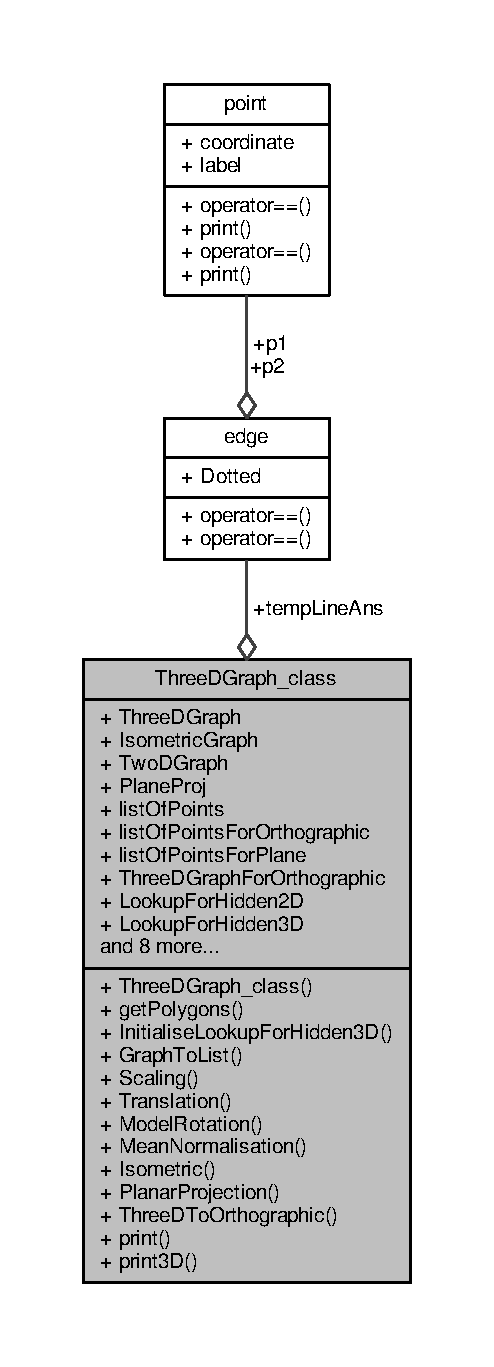
\includegraphics[height=550pt]{classThreeDGraph__class__coll__graph}
\end{center}
\end{figure}
\subsection*{Public Member Functions}
\begin{DoxyCompactItemize}
\item 
vector$<$ vector$<$ \hyperlink{structedge}{edge} $>$ $>$ \hyperlink{classThreeDGraph__class_a6bc32a5861610e120135f76383cbc8aa}{get\+Polygons} (bool ch)
\begin{DoxyCompactList}\small\item\em A Member function. \end{DoxyCompactList}\item 
void \hyperlink{classThreeDGraph__class_a132845f27333d0c2ead3a27bb4398a4d}{Initialise\+Lookup\+For\+Hidden3D} (bool Iso\+Or3D)
\begin{DoxyCompactList}\small\item\em A Member function. \end{DoxyCompactList}\item 
void \hyperlink{classThreeDGraph__class_a521cb31c72fa3828840a3bf4403e1395}{Graph\+To\+List} (bool Three\+D\+Graph\+Or\+Plane\+Proj)
\begin{DoxyCompactList}\small\item\em A Member function. \end{DoxyCompactList}\item 
void \hyperlink{classThreeDGraph__class_afa131e00002ddff96be961a903e2c589}{Scaling} (float Scale\+Factor)
\begin{DoxyCompactList}\small\item\em A Member function. \end{DoxyCompactList}\item 
void \hyperlink{classThreeDGraph__class_aa3f177ba316ff1fc411926ba9d08c80f}{Translation} (float x, float y, float z, \hyperlink{structedge}{edge} line, bool Graph\+Or\+Line)
\begin{DoxyCompactList}\small\item\em A Member function. \end{DoxyCompactList}\item 
void \hyperlink{classThreeDGraph__class_a400bececda29db8682455d92872f0a5e}{Model\+Rotation} (float angle, \hyperlink{structedge}{edge} axis)
\begin{DoxyCompactList}\small\item\em A Member function. \end{DoxyCompactList}\item 
void \hyperlink{classThreeDGraph__class_ad30f5f058cfe9a0de8a91dd062fb10c5}{Mean\+Normalisation} ()
\begin{DoxyCompactList}\small\item\em A Member function. \end{DoxyCompactList}\item 
void \hyperlink{classThreeDGraph__class_aec760645bb97742c87a50fe66aa68efe}{Isometric} ()
\begin{DoxyCompactList}\small\item\em A Member function. \end{DoxyCompactList}\item 
map$<$ string, vector$<$ \hyperlink{structpoint}{point} $>$ $>$ \hyperlink{classThreeDGraph__class_a9c802d66d5c79dd867f3566348d49921}{Planar\+Projection} (\hyperlink{structplane}{plane} equation\+Of\+Plane)
\begin{DoxyCompactList}\small\item\em A Member function. \end{DoxyCompactList}\item 
void \hyperlink{classThreeDGraph__class_ae69c2ee22498d903d1afa6b988edd1b6}{Three\+D\+To\+Orthographic} ()
\begin{DoxyCompactList}\small\item\em A Member function. \end{DoxyCompactList}\item 
void \hyperlink{classThreeDGraph__class_af53c26ef3f673e77e1213789fe14c8a2}{print} ()
\begin{DoxyCompactList}\small\item\em A Member function. \end{DoxyCompactList}\item 
void \hyperlink{classThreeDGraph__class_a08a1a3131c7090b8f783809f07810725}{print3D} ()
\begin{DoxyCompactList}\small\item\em A Member function. \end{DoxyCompactList}\end{DoxyCompactItemize}
\subsection*{Public Attributes}
\begin{DoxyCompactItemize}
\item 
map$<$ string, vector$<$ \hyperlink{structpoint}{point} $>$ $>$ \hyperlink{classThreeDGraph__class_a10f2244053d72def3eed9fb4101f0236}{Three\+D\+Graph}
\item 
map$<$ string, vector$<$ \hyperlink{structpoint}{point} $>$ $>$ \hyperlink{classThreeDGraph__class_afa3f00ec2a3864317ad121d087c9896d}{Isometric\+Graph}
\item 
map$<$ string, vector$<$ \hyperlink{structpoint}{point} $>$ $>$ \hyperlink{classThreeDGraph__class_a352d2c3b25256d8a071132dd87606f99}{Two\+D\+Graph} \mbox{[}3\mbox{]}
\item 
map$<$ string, vector$<$ \hyperlink{structpoint}{point} $>$ $>$ \hyperlink{classThreeDGraph__class_ad800b572d58a46cbd5b4139b3ec7b173}{Plane\+Proj}
\item 
vector$<$ string $>$ \hyperlink{classThreeDGraph__class_ab24656328d4be1eae0f6f5742add5969}{list\+Of\+Points}
\item 
vector$<$ string $>$ \hyperlink{classThreeDGraph__class_a9b5605ee14d7774be307a78d00930bd2}{list\+Of\+Points\+For\+Orthographic}
\item 
vector$<$ string $>$ \hyperlink{classThreeDGraph__class_a7a63687d665e48d41867a293d5d8bc16}{list\+Of\+Points\+For\+Plane}
\item 
map$<$ string, vector$<$ \hyperlink{structpoint}{point} $>$ $>$ \hyperlink{classThreeDGraph__class_a8099559641e72dbbd7e29e97f32dc242}{Three\+D\+Graph\+For\+Orthographic}
\item 
map$<$ string, vector$<$ bool $>$ $>$ \hyperlink{classThreeDGraph__class_a8b4c56978bacc0a509d5d69bf79c7125}{Lookup\+For\+Hidden2D} \mbox{[}3\mbox{]}
\item 
map$<$ string, vector$<$ bool $>$ $>$ \hyperlink{classThreeDGraph__class_ac32d99fa519519003b2e4658922afbe0}{Lookup\+For\+Hidden3D}
\item 
vector$<$ vector$<$ \hyperlink{structedge}{edge} $>$ $>$ \hyperlink{classThreeDGraph__class_a36fbc76142278359f5de0df528394944}{Face\+Graph}
\item 
Mat \hyperlink{classThreeDGraph__class_a52564aaa0f2223a754dccb28b347b009}{matrix\+Ans}
\item 
Mat \hyperlink{classThreeDGraph__class_a276acab9cffc9952e64514aad293da84}{matrix} \mbox{[}3\mbox{]}
\item 
Mat \hyperlink{classThreeDGraph__class_a03032b7bde495a752d3ccf43c3328f78}{matrixA}
\item 
Mat \hyperlink{classThreeDGraph__class_a487c0f52b65d943a04cf75077ab6b5fe}{matrixB}
\item 
\hyperlink{structedge}{edge} \hyperlink{classThreeDGraph__class_aa7a987df28f93f04fa0021d56a364a98}{temp\+Line\+Ans}
\item 
Vec \hyperlink{classThreeDGraph__class_a48d310a18f7602769320d2dae4445d25}{temp\+Line\+Vect}
\item 
Vec \hyperlink{classThreeDGraph__class_a68fb902385d303dcfcd1d9b0afd935cb}{temp\+Line\+Vect\+For\+Plane}
\item 
vector$<$ char $>$ \hyperlink{classThreeDGraph__class_a70ca0daf8f7348661bb3a429a10cf79a}{digit}
\end{DoxyCompactItemize}


\subsection{Detailed Description}
3D behaviour class. 

This class has all the functionalities that a 3D object can possess in the software. It can be rotated, projected along some plane or can give its orthographic projections 

\subsection{Member Function Documentation}
\index{Three\+D\+Graph\+\_\+class@{Three\+D\+Graph\+\_\+class}!get\+Polygons@{get\+Polygons}}
\index{get\+Polygons@{get\+Polygons}!Three\+D\+Graph\+\_\+class@{Three\+D\+Graph\+\_\+class}}
\subsubsection[{\texorpdfstring{get\+Polygons(bool ch)}{getPolygons(bool ch)}}]{\setlength{\rightskip}{0pt plus 5cm}vector$<$ vector$<$ {\bf edge} $>$ $>$ Three\+D\+Graph\+\_\+class\+::get\+Polygons (
\begin{DoxyParamCaption}
\item[{bool}]{ch}
\end{DoxyParamCaption}
)}\hypertarget{classThreeDGraph__class_a6bc32a5861610e120135f76383cbc8aa}{}\label{classThreeDGraph__class_a6bc32a5861610e120135f76383cbc8aa}


A Member function. 


\begin{DoxyParams}{Parameters}
{\em ch} & a boolean argument to recognize whether we have to recignize faces of our 3D graph/ Isometric graph Function to recognize faces in a graph \\
\hline
\end{DoxyParams}
\index{Three\+D\+Graph\+\_\+class@{Three\+D\+Graph\+\_\+class}!Graph\+To\+List@{Graph\+To\+List}}
\index{Graph\+To\+List@{Graph\+To\+List}!Three\+D\+Graph\+\_\+class@{Three\+D\+Graph\+\_\+class}}
\subsubsection[{\texorpdfstring{Graph\+To\+List(bool Three\+D\+Graph\+Or\+Plane\+Proj)}{GraphToList(bool ThreeDGraphOrPlaneProj)}}]{\setlength{\rightskip}{0pt plus 5cm}void Three\+D\+Graph\+\_\+class\+::\+Graph\+To\+List (
\begin{DoxyParamCaption}
\item[{bool}]{Three\+D\+Graph\+Or\+Plane\+Proj}
\end{DoxyParamCaption}
)}\hypertarget{classThreeDGraph__class_a521cb31c72fa3828840a3bf4403e1395}{}\label{classThreeDGraph__class_a521cb31c72fa3828840a3bf4403e1395}


A Member function. 

Function to create list\+Of\+Points for 3D graph \index{Three\+D\+Graph\+\_\+class@{Three\+D\+Graph\+\_\+class}!Initialise\+Lookup\+For\+Hidden3D@{Initialise\+Lookup\+For\+Hidden3D}}
\index{Initialise\+Lookup\+For\+Hidden3D@{Initialise\+Lookup\+For\+Hidden3D}!Three\+D\+Graph\+\_\+class@{Three\+D\+Graph\+\_\+class}}
\subsubsection[{\texorpdfstring{Initialise\+Lookup\+For\+Hidden3\+D(bool Iso\+Or3\+D)}{InitialiseLookupForHidden3D(bool IsoOr3D)}}]{\setlength{\rightskip}{0pt plus 5cm}void Three\+D\+Graph\+\_\+class\+::\+Initialise\+Lookup\+For\+Hidden3D (
\begin{DoxyParamCaption}
\item[{bool}]{Iso\+Or3D}
\end{DoxyParamCaption}
)}\hypertarget{classThreeDGraph__class_a132845f27333d0c2ead3a27bb4398a4d}{}\label{classThreeDGraph__class_a132845f27333d0c2ead3a27bb4398a4d}


A Member function. 

Function to initialise a lookup vector to list\+Of\+Points for 3D graph \index{Three\+D\+Graph\+\_\+class@{Three\+D\+Graph\+\_\+class}!Isometric@{Isometric}}
\index{Isometric@{Isometric}!Three\+D\+Graph\+\_\+class@{Three\+D\+Graph\+\_\+class}}
\subsubsection[{\texorpdfstring{Isometric()}{Isometric()}}]{\setlength{\rightskip}{0pt plus 5cm}void Three\+D\+Graph\+\_\+class\+::\+Isometric (
\begin{DoxyParamCaption}
{}
\end{DoxyParamCaption}
)}\hypertarget{classThreeDGraph__class_aec760645bb97742c87a50fe66aa68efe}{}\label{classThreeDGraph__class_aec760645bb97742c87a50fe66aa68efe}


A Member function. 

A function to get Isometric graoh from 3D graph \index{Three\+D\+Graph\+\_\+class@{Three\+D\+Graph\+\_\+class}!Mean\+Normalisation@{Mean\+Normalisation}}
\index{Mean\+Normalisation@{Mean\+Normalisation}!Three\+D\+Graph\+\_\+class@{Three\+D\+Graph\+\_\+class}}
\subsubsection[{\texorpdfstring{Mean\+Normalisation()}{MeanNormalisation()}}]{\setlength{\rightskip}{0pt plus 5cm}void Three\+D\+Graph\+\_\+class\+::\+Mean\+Normalisation (
\begin{DoxyParamCaption}
{}
\end{DoxyParamCaption}
)}\hypertarget{classThreeDGraph__class_ad30f5f058cfe9a0de8a91dd062fb10c5}{}\label{classThreeDGraph__class_ad30f5f058cfe9a0de8a91dd062fb10c5}


A Member function. 

A function to scale and translate our object to origin and scale it to look good on canvas \index{Three\+D\+Graph\+\_\+class@{Three\+D\+Graph\+\_\+class}!Model\+Rotation@{Model\+Rotation}}
\index{Model\+Rotation@{Model\+Rotation}!Three\+D\+Graph\+\_\+class@{Three\+D\+Graph\+\_\+class}}
\subsubsection[{\texorpdfstring{Model\+Rotation(float angle, edge axis)}{ModelRotation(float angle, edge axis)}}]{\setlength{\rightskip}{0pt plus 5cm}void Three\+D\+Graph\+\_\+class\+::\+Model\+Rotation (
\begin{DoxyParamCaption}
\item[{float}]{angle, }
\item[{{\bf edge}}]{axis}
\end{DoxyParamCaption}
)}\hypertarget{classThreeDGraph__class_a400bececda29db8682455d92872f0a5e}{}\label{classThreeDGraph__class_a400bececda29db8682455d92872f0a5e}


A Member function. 


\begin{DoxyParams}{Parameters}
{\em angle} & a float argument to tell the angle of rotation. \\
\hline
{\em exis} & an edge about which we have to rotate. A function to rotate a graph about an axis by an angle \\
\hline
\end{DoxyParams}
\index{Three\+D\+Graph\+\_\+class@{Three\+D\+Graph\+\_\+class}!Planar\+Projection@{Planar\+Projection}}
\index{Planar\+Projection@{Planar\+Projection}!Three\+D\+Graph\+\_\+class@{Three\+D\+Graph\+\_\+class}}
\subsubsection[{\texorpdfstring{Planar\+Projection(plane equation\+Of\+Plane)}{PlanarProjection(plane equationOfPlane)}}]{\setlength{\rightskip}{0pt plus 5cm}map$<$ string, vector$<$ {\bf point} $>$ $>$ Three\+D\+Graph\+\_\+class\+::\+Planar\+Projection (
\begin{DoxyParamCaption}
\item[{{\bf plane}}]{equation\+Of\+Plane}
\end{DoxyParamCaption}
)}\hypertarget{classThreeDGraph__class_a9c802d66d5c79dd867f3566348d49921}{}\label{classThreeDGraph__class_a9c802d66d5c79dd867f3566348d49921}


A Member function. 

\begin{DoxySeeAlso}{See also}
\hyperlink{classThreeDGraph__class_a521cb31c72fa3828840a3bf4403e1395}{Graph\+To\+List()} 
\end{DoxySeeAlso}

\begin{DoxyParams}{Parameters}
{\em equation\+Of\+Plane} & this defines the plane on which projection has to be taken. A function to get a plane projection of a 3D graph on a plane \\
\hline
\end{DoxyParams}
\index{Three\+D\+Graph\+\_\+class@{Three\+D\+Graph\+\_\+class}!print@{print}}
\index{print@{print}!Three\+D\+Graph\+\_\+class@{Three\+D\+Graph\+\_\+class}}
\subsubsection[{\texorpdfstring{print()}{print()}}]{\setlength{\rightskip}{0pt plus 5cm}void Three\+D\+Graph\+\_\+class\+::print (
\begin{DoxyParamCaption}
{}
\end{DoxyParamCaption}
)}\hypertarget{classThreeDGraph__class_af53c26ef3f673e77e1213789fe14c8a2}{}\label{classThreeDGraph__class_af53c26ef3f673e77e1213789fe14c8a2}


A Member function. 

Function to print 2D graph of Y-\/Z plane on terminal for debugging purposes \index{Three\+D\+Graph\+\_\+class@{Three\+D\+Graph\+\_\+class}!print3D@{print3D}}
\index{print3D@{print3D}!Three\+D\+Graph\+\_\+class@{Three\+D\+Graph\+\_\+class}}
\subsubsection[{\texorpdfstring{print3\+D()}{print3D()}}]{\setlength{\rightskip}{0pt plus 5cm}void Three\+D\+Graph\+\_\+class\+::print3D (
\begin{DoxyParamCaption}
{}
\end{DoxyParamCaption}
)}\hypertarget{classThreeDGraph__class_a08a1a3131c7090b8f783809f07810725}{}\label{classThreeDGraph__class_a08a1a3131c7090b8f783809f07810725}


A Member function. 

Function to print 3D graph on terminal for debugging purposes \index{Three\+D\+Graph\+\_\+class@{Three\+D\+Graph\+\_\+class}!Scaling@{Scaling}}
\index{Scaling@{Scaling}!Three\+D\+Graph\+\_\+class@{Three\+D\+Graph\+\_\+class}}
\subsubsection[{\texorpdfstring{Scaling(float Scale\+Factor)}{Scaling(float ScaleFactor)}}]{\setlength{\rightskip}{0pt plus 5cm}void Three\+D\+Graph\+\_\+class\+::\+Scaling (
\begin{DoxyParamCaption}
\item[{float}]{Scale\+Factor}
\end{DoxyParamCaption}
)}\hypertarget{classThreeDGraph__class_afa131e00002ddff96be961a903e2c589}{}\label{classThreeDGraph__class_afa131e00002ddff96be961a903e2c589}


A Member function. 


\begin{DoxyParams}{Parameters}
{\em Scale\+Factor} & to tell the factor of scale. Will scale the graph to the scale factor \\
\hline
\end{DoxyParams}
\index{Three\+D\+Graph\+\_\+class@{Three\+D\+Graph\+\_\+class}!Three\+D\+To\+Orthographic@{Three\+D\+To\+Orthographic}}
\index{Three\+D\+To\+Orthographic@{Three\+D\+To\+Orthographic}!Three\+D\+Graph\+\_\+class@{Three\+D\+Graph\+\_\+class}}
\subsubsection[{\texorpdfstring{Three\+D\+To\+Orthographic()}{ThreeDToOrthographic()}}]{\setlength{\rightskip}{0pt plus 5cm}void Three\+D\+Graph\+\_\+class\+::\+Three\+D\+To\+Orthographic (
\begin{DoxyParamCaption}
{}
\end{DoxyParamCaption}
)}\hypertarget{classThreeDGraph__class_ae69c2ee22498d903d1afa6b988edd1b6}{}\label{classThreeDGraph__class_ae69c2ee22498d903d1afa6b988edd1b6}


A Member function. 

A function to create all 3 orthographic projections from a 3D graph and save them in a 2D graph \index{Three\+D\+Graph\+\_\+class@{Three\+D\+Graph\+\_\+class}!Translation@{Translation}}
\index{Translation@{Translation}!Three\+D\+Graph\+\_\+class@{Three\+D\+Graph\+\_\+class}}
\subsubsection[{\texorpdfstring{Translation(float x, float y, float z, edge line, bool Graph\+Or\+Line)}{Translation(float x, float y, float z, edge line, bool GraphOrLine)}}]{\setlength{\rightskip}{0pt plus 5cm}void Three\+D\+Graph\+\_\+class\+::\+Translation (
\begin{DoxyParamCaption}
\item[{float}]{x, }
\item[{float}]{y, }
\item[{float}]{z, }
\item[{{\bf edge}}]{line, }
\item[{bool}]{Graph\+Or\+Line}
\end{DoxyParamCaption}
)}\hypertarget{classThreeDGraph__class_aa3f177ba316ff1fc411926ba9d08c80f}{}\label{classThreeDGraph__class_aa3f177ba316ff1fc411926ba9d08c80f}


A Member function. 

\begin{DoxySeeAlso}{See also}
\hyperlink{classThreeDGraph__class_aa3f177ba316ff1fc411926ba9d08c80f}{Translation()} 
\end{DoxySeeAlso}

\begin{DoxyParams}{Parameters}
{\em x} & to tell the amount of shift in x coordinate. \\
\hline
{\em y} & to tell the amount of shift in y coordinate. \\
\hline
{\em z} & to tell the amount of shift in z coordinate. \\
\hline
{\em line} & line to translate. \\
\hline
{\em Graph\+Or\+Line} & boolean character to tell whether translation required is of line or graph. A function to translate the graph to specified position \\
\hline
\end{DoxyParams}


\subsection{Member Data Documentation}
\index{Three\+D\+Graph\+\_\+class@{Three\+D\+Graph\+\_\+class}!digit@{digit}}
\index{digit@{digit}!Three\+D\+Graph\+\_\+class@{Three\+D\+Graph\+\_\+class}}
\subsubsection[{\texorpdfstring{digit}{digit}}]{\setlength{\rightskip}{0pt plus 5cm}vector$<$char$>$ Three\+D\+Graph\+\_\+class\+::digit}\hypertarget{classThreeDGraph__class_a70ca0daf8f7348661bb3a429a10cf79a}{}\label{classThreeDGraph__class_a70ca0daf8f7348661bb3a429a10cf79a}
To store the coincident labels in a view for a particular vertex \index{Three\+D\+Graph\+\_\+class@{Three\+D\+Graph\+\_\+class}!Face\+Graph@{Face\+Graph}}
\index{Face\+Graph@{Face\+Graph}!Three\+D\+Graph\+\_\+class@{Three\+D\+Graph\+\_\+class}}
\subsubsection[{\texorpdfstring{Face\+Graph}{FaceGraph}}]{\setlength{\rightskip}{0pt plus 5cm}vector$<$ vector$<$ {\bf edge}$>$ $>$ Three\+D\+Graph\+\_\+class\+::\+Face\+Graph}\hypertarget{classThreeDGraph__class_a36fbc76142278359f5de0df528394944}{}\label{classThreeDGraph__class_a36fbc76142278359f5de0df528394944}
This is the graph containing faces and corresponding edges on them \index{Three\+D\+Graph\+\_\+class@{Three\+D\+Graph\+\_\+class}!Isometric\+Graph@{Isometric\+Graph}}
\index{Isometric\+Graph@{Isometric\+Graph}!Three\+D\+Graph\+\_\+class@{Three\+D\+Graph\+\_\+class}}
\subsubsection[{\texorpdfstring{Isometric\+Graph}{IsometricGraph}}]{\setlength{\rightskip}{0pt plus 5cm}map$<$string, vector$<${\bf point}$>$ $>$ Three\+D\+Graph\+\_\+class\+::\+Isometric\+Graph}\hypertarget{classThreeDGraph__class_afa3f00ec2a3864317ad121d087c9896d}{}\label{classThreeDGraph__class_afa3f00ec2a3864317ad121d087c9896d}
This is the Isometric graph representation \index{Three\+D\+Graph\+\_\+class@{Three\+D\+Graph\+\_\+class}!list\+Of\+Points@{list\+Of\+Points}}
\index{list\+Of\+Points@{list\+Of\+Points}!Three\+D\+Graph\+\_\+class@{Three\+D\+Graph\+\_\+class}}
\subsubsection[{\texorpdfstring{list\+Of\+Points}{listOfPoints}}]{\setlength{\rightskip}{0pt plus 5cm}vector$<$string$>$ Three\+D\+Graph\+\_\+class\+::list\+Of\+Points}\hypertarget{classThreeDGraph__class_ab24656328d4be1eae0f6f5742add5969}{}\label{classThreeDGraph__class_ab24656328d4be1eae0f6f5742add5969}
This is list of points available in 3D graph \index{Three\+D\+Graph\+\_\+class@{Three\+D\+Graph\+\_\+class}!list\+Of\+Points\+For\+Orthographic@{list\+Of\+Points\+For\+Orthographic}}
\index{list\+Of\+Points\+For\+Orthographic@{list\+Of\+Points\+For\+Orthographic}!Three\+D\+Graph\+\_\+class@{Three\+D\+Graph\+\_\+class}}
\subsubsection[{\texorpdfstring{list\+Of\+Points\+For\+Orthographic}{listOfPointsForOrthographic}}]{\setlength{\rightskip}{0pt plus 5cm}vector$<$string$>$ Three\+D\+Graph\+\_\+class\+::list\+Of\+Points\+For\+Orthographic}\hypertarget{classThreeDGraph__class_a9b5605ee14d7774be307a78d00930bd2}{}\label{classThreeDGraph__class_a9b5605ee14d7774be307a78d00930bd2}
This is list of points available for a particular orthographic projection \index{Three\+D\+Graph\+\_\+class@{Three\+D\+Graph\+\_\+class}!list\+Of\+Points\+For\+Plane@{list\+Of\+Points\+For\+Plane}}
\index{list\+Of\+Points\+For\+Plane@{list\+Of\+Points\+For\+Plane}!Three\+D\+Graph\+\_\+class@{Three\+D\+Graph\+\_\+class}}
\subsubsection[{\texorpdfstring{list\+Of\+Points\+For\+Plane}{listOfPointsForPlane}}]{\setlength{\rightskip}{0pt plus 5cm}vector$<$string$>$ Three\+D\+Graph\+\_\+class\+::list\+Of\+Points\+For\+Plane}\hypertarget{classThreeDGraph__class_a7a63687d665e48d41867a293d5d8bc16}{}\label{classThreeDGraph__class_a7a63687d665e48d41867a293d5d8bc16}
This is list of points available in planar Projection \index{Three\+D\+Graph\+\_\+class@{Three\+D\+Graph\+\_\+class}!Lookup\+For\+Hidden2D@{Lookup\+For\+Hidden2D}}
\index{Lookup\+For\+Hidden2D@{Lookup\+For\+Hidden2D}!Three\+D\+Graph\+\_\+class@{Three\+D\+Graph\+\_\+class}}
\subsubsection[{\texorpdfstring{Lookup\+For\+Hidden2D}{LookupForHidden2D}}]{\setlength{\rightskip}{0pt plus 5cm}map$<$string, vector$<$bool$>$ $>$ Three\+D\+Graph\+\_\+class\+::\+Lookup\+For\+Hidden2D\mbox{[}3\mbox{]}}\hypertarget{classThreeDGraph__class_a8b4c56978bacc0a509d5d69bf79c7125}{}\label{classThreeDGraph__class_a8b4c56978bacc0a509d5d69bf79c7125}
This is orthographic projections hidden edges \index{Three\+D\+Graph\+\_\+class@{Three\+D\+Graph\+\_\+class}!Lookup\+For\+Hidden3D@{Lookup\+For\+Hidden3D}}
\index{Lookup\+For\+Hidden3D@{Lookup\+For\+Hidden3D}!Three\+D\+Graph\+\_\+class@{Three\+D\+Graph\+\_\+class}}
\subsubsection[{\texorpdfstring{Lookup\+For\+Hidden3D}{LookupForHidden3D}}]{\setlength{\rightskip}{0pt plus 5cm}map$<$string, vector$<$bool$>$ $>$ Three\+D\+Graph\+\_\+class\+::\+Lookup\+For\+Hidden3D}\hypertarget{classThreeDGraph__class_ac32d99fa519519003b2e4658922afbe0}{}\label{classThreeDGraph__class_ac32d99fa519519003b2e4658922afbe0}
This is the 3D graph representation of hidden edges \index{Three\+D\+Graph\+\_\+class@{Three\+D\+Graph\+\_\+class}!matrix@{matrix}}
\index{matrix@{matrix}!Three\+D\+Graph\+\_\+class@{Three\+D\+Graph\+\_\+class}}
\subsubsection[{\texorpdfstring{matrix}{matrix}}]{\setlength{\rightskip}{0pt plus 5cm}Mat Three\+D\+Graph\+\_\+class\+::matrix\mbox{[}3\mbox{]}}\hypertarget{classThreeDGraph__class_a276acab9cffc9952e64514aad293da84}{}\label{classThreeDGraph__class_a276acab9cffc9952e64514aad293da84}
This is matrix for rotating about specific axis \index{Three\+D\+Graph\+\_\+class@{Three\+D\+Graph\+\_\+class}!matrixA@{matrixA}}
\index{matrixA@{matrixA}!Three\+D\+Graph\+\_\+class@{Three\+D\+Graph\+\_\+class}}
\subsubsection[{\texorpdfstring{matrixA}{matrixA}}]{\setlength{\rightskip}{0pt plus 5cm}Mat Three\+D\+Graph\+\_\+class\+::matrixA}\hypertarget{classThreeDGraph__class_a03032b7bde495a752d3ccf43c3328f78}{}\label{classThreeDGraph__class_a03032b7bde495a752d3ccf43c3328f78}
This is matrix for rotating about specific axis \index{Three\+D\+Graph\+\_\+class@{Three\+D\+Graph\+\_\+class}!matrix\+Ans@{matrix\+Ans}}
\index{matrix\+Ans@{matrix\+Ans}!Three\+D\+Graph\+\_\+class@{Three\+D\+Graph\+\_\+class}}
\subsubsection[{\texorpdfstring{matrix\+Ans}{matrixAns}}]{\setlength{\rightskip}{0pt plus 5cm}Mat Three\+D\+Graph\+\_\+class\+::matrix\+Ans}\hypertarget{classThreeDGraph__class_a52564aaa0f2223a754dccb28b347b009}{}\label{classThreeDGraph__class_a52564aaa0f2223a754dccb28b347b009}
This is answer calculated after matrix computations \index{Three\+D\+Graph\+\_\+class@{Three\+D\+Graph\+\_\+class}!matrixB@{matrixB}}
\index{matrixB@{matrixB}!Three\+D\+Graph\+\_\+class@{Three\+D\+Graph\+\_\+class}}
\subsubsection[{\texorpdfstring{matrixB}{matrixB}}]{\setlength{\rightskip}{0pt plus 5cm}Mat Three\+D\+Graph\+\_\+class\+::matrixB}\hypertarget{classThreeDGraph__class_a487c0f52b65d943a04cf75077ab6b5fe}{}\label{classThreeDGraph__class_a487c0f52b65d943a04cf75077ab6b5fe}
This is matrix for rotating about specific axis \index{Three\+D\+Graph\+\_\+class@{Three\+D\+Graph\+\_\+class}!Plane\+Proj@{Plane\+Proj}}
\index{Plane\+Proj@{Plane\+Proj}!Three\+D\+Graph\+\_\+class@{Three\+D\+Graph\+\_\+class}}
\subsubsection[{\texorpdfstring{Plane\+Proj}{PlaneProj}}]{\setlength{\rightskip}{0pt plus 5cm}map$<$string, vector$<${\bf point}$>$ $>$ Three\+D\+Graph\+\_\+class\+::\+Plane\+Proj}\hypertarget{classThreeDGraph__class_ad800b572d58a46cbd5b4139b3ec7b173}{}\label{classThreeDGraph__class_ad800b572d58a46cbd5b4139b3ec7b173}
This is planar projection of 3D graph when requested \index{Three\+D\+Graph\+\_\+class@{Three\+D\+Graph\+\_\+class}!temp\+Line\+Ans@{temp\+Line\+Ans}}
\index{temp\+Line\+Ans@{temp\+Line\+Ans}!Three\+D\+Graph\+\_\+class@{Three\+D\+Graph\+\_\+class}}
\subsubsection[{\texorpdfstring{temp\+Line\+Ans}{tempLineAns}}]{\setlength{\rightskip}{0pt plus 5cm}{\bf edge} Three\+D\+Graph\+\_\+class\+::temp\+Line\+Ans}\hypertarget{classThreeDGraph__class_aa7a987df28f93f04fa0021d56a364a98}{}\label{classThreeDGraph__class_aa7a987df28f93f04fa0021d56a364a98}
This is an temporary edge \index{Three\+D\+Graph\+\_\+class@{Three\+D\+Graph\+\_\+class}!temp\+Line\+Vect@{temp\+Line\+Vect}}
\index{temp\+Line\+Vect@{temp\+Line\+Vect}!Three\+D\+Graph\+\_\+class@{Three\+D\+Graph\+\_\+class}}
\subsubsection[{\texorpdfstring{temp\+Line\+Vect}{tempLineVect}}]{\setlength{\rightskip}{0pt plus 5cm}Vec Three\+D\+Graph\+\_\+class\+::temp\+Line\+Vect}\hypertarget{classThreeDGraph__class_a48d310a18f7602769320d2dae4445d25}{}\label{classThreeDGraph__class_a48d310a18f7602769320d2dae4445d25}
This is a temporary vector \index{Three\+D\+Graph\+\_\+class@{Three\+D\+Graph\+\_\+class}!temp\+Line\+Vect\+For\+Plane@{temp\+Line\+Vect\+For\+Plane}}
\index{temp\+Line\+Vect\+For\+Plane@{temp\+Line\+Vect\+For\+Plane}!Three\+D\+Graph\+\_\+class@{Three\+D\+Graph\+\_\+class}}
\subsubsection[{\texorpdfstring{temp\+Line\+Vect\+For\+Plane}{tempLineVectForPlane}}]{\setlength{\rightskip}{0pt plus 5cm}Vec Three\+D\+Graph\+\_\+class\+::temp\+Line\+Vect\+For\+Plane}\hypertarget{classThreeDGraph__class_a68fb902385d303dcfcd1d9b0afd935cb}{}\label{classThreeDGraph__class_a68fb902385d303dcfcd1d9b0afd935cb}
This is a temporary vector \index{Three\+D\+Graph\+\_\+class@{Three\+D\+Graph\+\_\+class}!Three\+D\+Graph@{Three\+D\+Graph}}
\index{Three\+D\+Graph@{Three\+D\+Graph}!Three\+D\+Graph\+\_\+class@{Three\+D\+Graph\+\_\+class}}
\subsubsection[{\texorpdfstring{Three\+D\+Graph}{ThreeDGraph}}]{\setlength{\rightskip}{0pt plus 5cm}map$<$string, vector$<${\bf point}$>$ $>$ Three\+D\+Graph\+\_\+class\+::\+Three\+D\+Graph}\hypertarget{classThreeDGraph__class_a10f2244053d72def3eed9fb4101f0236}{}\label{classThreeDGraph__class_a10f2244053d72def3eed9fb4101f0236}
This is the 3D graph representation \index{Three\+D\+Graph\+\_\+class@{Three\+D\+Graph\+\_\+class}!Three\+D\+Graph\+For\+Orthographic@{Three\+D\+Graph\+For\+Orthographic}}
\index{Three\+D\+Graph\+For\+Orthographic@{Three\+D\+Graph\+For\+Orthographic}!Three\+D\+Graph\+\_\+class@{Three\+D\+Graph\+\_\+class}}
\subsubsection[{\texorpdfstring{Three\+D\+Graph\+For\+Orthographic}{ThreeDGraphForOrthographic}}]{\setlength{\rightskip}{0pt plus 5cm}map$<$string, vector$<${\bf point}$>$ $>$ Three\+D\+Graph\+\_\+class\+::\+Three\+D\+Graph\+For\+Orthographic}\hypertarget{classThreeDGraph__class_a8099559641e72dbbd7e29e97f32dc242}{}\label{classThreeDGraph__class_a8099559641e72dbbd7e29e97f32dc242}
This is the 3D graph representation \index{Three\+D\+Graph\+\_\+class@{Three\+D\+Graph\+\_\+class}!Two\+D\+Graph@{Two\+D\+Graph}}
\index{Two\+D\+Graph@{Two\+D\+Graph}!Three\+D\+Graph\+\_\+class@{Three\+D\+Graph\+\_\+class}}
\subsubsection[{\texorpdfstring{Two\+D\+Graph}{TwoDGraph}}]{\setlength{\rightskip}{0pt plus 5cm}map$<$string, vector$<${\bf point}$>$ $>$ Three\+D\+Graph\+\_\+class\+::\+Two\+D\+Graph\mbox{[}3\mbox{]}}\hypertarget{classThreeDGraph__class_a352d2c3b25256d8a071132dd87606f99}{}\label{classThreeDGraph__class_a352d2c3b25256d8a071132dd87606f99}
This is orthographic projections 

The documentation for this class was generated from the following files\+:\begin{DoxyCompactItemize}
\item 
Include/\hyperlink{3DProcessingSrc_8h}{3\+D\+Processing\+Src.\+h}\item 
Src/\hyperlink{3DProcessingSrc_8cpp}{3\+D\+Processing\+Src.\+cpp}\end{DoxyCompactItemize}

\hypertarget{classTwoDGraph__class}{}\section{Two\+D\+Graph\+\_\+class Class Reference}
\label{classTwoDGraph__class}\index{Two\+D\+Graph\+\_\+class@{Two\+D\+Graph\+\_\+class}}


2D behaviour class.  




Collaboration diagram for Two\+D\+Graph\+\_\+class\+:
\nopagebreak
\begin{figure}[H]
\begin{center}
\leavevmode
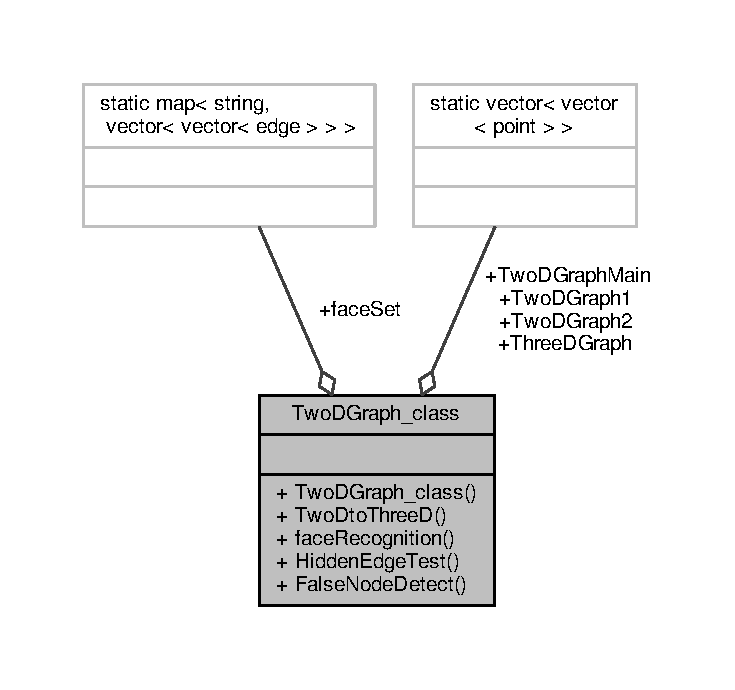
\includegraphics[width=350pt]{classTwoDGraph__class__coll__graph}
\end{center}
\end{figure}
\subsection*{Public Member Functions}
\begin{DoxyCompactItemize}
\item 
\hyperlink{classTwoDGraph__class_aa666c42d1e81f8da8cc9229f46c572f5}{Two\+D\+Graph\+\_\+class} (vector$<$ vector$<$ \hyperlink{structpoint}{point} $>$ $>$ graph1, vector$<$ vector$<$ \hyperlink{structpoint}{point} $>$ $>$ graph2, vector$<$ vector$<$ \hyperlink{structpoint}{point} $>$ $>$ graph3)
\item 
void \hyperlink{classTwoDGraph__class_a48222790dda1c34caf1366ce1cc0ce1d}{Two\+Dto\+ThreeD} ()
\begin{DoxyCompactList}\small\item\em A Member function. \end{DoxyCompactList}\item 
void \hyperlink{classTwoDGraph__class_af0b7cb652fec315e79e0f4826c64ae6d}{face\+Recognition} ()
\begin{DoxyCompactList}\small\item\em A Member function. \end{DoxyCompactList}\item 
void \hyperlink{classTwoDGraph__class_a551441ccdbceddd7c5d7df8c3a0a3e04}{Hidden\+Edge\+Test} ()
\begin{DoxyCompactList}\small\item\em A Member function. \end{DoxyCompactList}\item 
void \hyperlink{classTwoDGraph__class_aac6062b9859be331a44d1fe61036d5a1}{False\+Node\+Detect} ()
\begin{DoxyCompactList}\small\item\em A Member function. \end{DoxyCompactList}\end{DoxyCompactItemize}
\subsection*{Static Public Attributes}
\begin{DoxyCompactItemize}
\item 
static vector$<$ vector$<$ \hyperlink{structpoint}{point} $>$ $>$ \hyperlink{classTwoDGraph__class_a973baa8979a298061224d1b949381a58}{Two\+D\+Graph\+Main}
\item 
static vector$<$ vector$<$ \hyperlink{structpoint}{point} $>$ $>$ \hyperlink{classTwoDGraph__class_a238b6e7f880ff95f27e21c951b54440b}{Two\+D\+Graph1}
\item 
static vector$<$ vector$<$ \hyperlink{structpoint}{point} $>$ $>$ \hyperlink{classTwoDGraph__class_aaedb57508908d5d956caa874e6a88505}{Two\+D\+Graph2}
\item 
static vector$<$ vector$<$ \hyperlink{structpoint}{point} $>$ $>$ \hyperlink{classTwoDGraph__class_a45b2a73d8f2a9ce4b72a2a6aaa8e2c4f}{Three\+D\+Graph}
\item 
static map$<$ string, vector$<$ vector$<$ \hyperlink{structedge}{edge} $>$ $>$ $>$ \hyperlink{classTwoDGraph__class_a80d22cc10e3cfa2d3f090bc0b506e2ea}{face\+Set}
\end{DoxyCompactItemize}


\subsection{Detailed Description}
2D behaviour class. 

This class has all the functionalities that a 2D object can possess in the software. It can be rotated and converted into isometric from 2 orthographic projections along some plane. 

\subsection{Constructor \& Destructor Documentation}
\index{Two\+D\+Graph\+\_\+class@{Two\+D\+Graph\+\_\+class}!Two\+D\+Graph\+\_\+class@{Two\+D\+Graph\+\_\+class}}
\index{Two\+D\+Graph\+\_\+class@{Two\+D\+Graph\+\_\+class}!Two\+D\+Graph\+\_\+class@{Two\+D\+Graph\+\_\+class}}
\subsubsection[{\texorpdfstring{Two\+D\+Graph\+\_\+class(vector$<$ vector$<$ point $>$ $>$ graph1, vector$<$ vector$<$ point $>$ $>$ graph2, vector$<$ vector$<$ point $>$ $>$ graph3)}{TwoDGraph_class(vector< vector< point > > graph1, vector< vector< point > > graph2, vector< vector< point > > graph3)}}]{\setlength{\rightskip}{0pt plus 5cm}Two\+D\+Graph\+\_\+class\+::\+Two\+D\+Graph\+\_\+class (
\begin{DoxyParamCaption}
\item[{vector$<$ vector$<$ {\bf point} $>$ $>$}]{graph1, }
\item[{vector$<$ vector$<$ {\bf point} $>$ $>$}]{graph2, }
\item[{vector$<$ vector$<$ {\bf point} $>$ $>$}]{graph3}
\end{DoxyParamCaption}
)\hspace{0.3cm}{\ttfamily [inline]}}\hypertarget{classTwoDGraph__class_aa666c42d1e81f8da8cc9229f46c572f5}{}\label{classTwoDGraph__class_aa666c42d1e81f8da8cc9229f46c572f5}


\subsection{Member Function Documentation}
\index{Two\+D\+Graph\+\_\+class@{Two\+D\+Graph\+\_\+class}!face\+Recognition@{face\+Recognition}}
\index{face\+Recognition@{face\+Recognition}!Two\+D\+Graph\+\_\+class@{Two\+D\+Graph\+\_\+class}}
\subsubsection[{\texorpdfstring{face\+Recognition()}{faceRecognition()}}]{\setlength{\rightskip}{0pt plus 5cm}void Two\+D\+Graph\+\_\+class\+::face\+Recognition (
\begin{DoxyParamCaption}
{}
\end{DoxyParamCaption}
)\hspace{0.3cm}{\ttfamily [inline]}}\hypertarget{classTwoDGraph__class_af0b7cb652fec315e79e0f4826c64ae6d}{}\label{classTwoDGraph__class_af0b7cb652fec315e79e0f4826c64ae6d}


A Member function. 

\begin{DoxySeeAlso}{See also}
\hyperlink{classTwoDGraph__class_af0b7cb652fec315e79e0f4826c64ae6d}{face\+Recognition()} 
\end{DoxySeeAlso}

\begin{DoxyParams}{Parameters}
{\em filename} & a string argument. \\
\hline
{\em flag3\+Dfile} & boolean character to tell the type of file (3\+D/2D). \\
\hline
\end{DoxyParams}
\index{Two\+D\+Graph\+\_\+class@{Two\+D\+Graph\+\_\+class}!False\+Node\+Detect@{False\+Node\+Detect}}
\index{False\+Node\+Detect@{False\+Node\+Detect}!Two\+D\+Graph\+\_\+class@{Two\+D\+Graph\+\_\+class}}
\subsubsection[{\texorpdfstring{False\+Node\+Detect()}{FalseNodeDetect()}}]{\setlength{\rightskip}{0pt plus 5cm}void Two\+D\+Graph\+\_\+class\+::\+False\+Node\+Detect (
\begin{DoxyParamCaption}
{}
\end{DoxyParamCaption}
)\hspace{0.3cm}{\ttfamily [inline]}}\hypertarget{classTwoDGraph__class_aac6062b9859be331a44d1fe61036d5a1}{}\label{classTwoDGraph__class_aac6062b9859be331a44d1fe61036d5a1}


A Member function. 

\begin{DoxySeeAlso}{See also}
\hyperlink{classTwoDGraph__class_aac6062b9859be331a44d1fe61036d5a1}{False\+Node\+Detect()} 
\end{DoxySeeAlso}

\begin{DoxyParams}{Parameters}
{\em filename} & a string argument. \\
\hline
{\em flag3\+Dfile} & boolean character to tell the type of file (3\+D/2D). \\
\hline
\end{DoxyParams}
\index{Two\+D\+Graph\+\_\+class@{Two\+D\+Graph\+\_\+class}!Hidden\+Edge\+Test@{Hidden\+Edge\+Test}}
\index{Hidden\+Edge\+Test@{Hidden\+Edge\+Test}!Two\+D\+Graph\+\_\+class@{Two\+D\+Graph\+\_\+class}}
\subsubsection[{\texorpdfstring{Hidden\+Edge\+Test()}{HiddenEdgeTest()}}]{\setlength{\rightskip}{0pt plus 5cm}void Two\+D\+Graph\+\_\+class\+::\+Hidden\+Edge\+Test (
\begin{DoxyParamCaption}
{}
\end{DoxyParamCaption}
)\hspace{0.3cm}{\ttfamily [inline]}}\hypertarget{classTwoDGraph__class_a551441ccdbceddd7c5d7df8c3a0a3e04}{}\label{classTwoDGraph__class_a551441ccdbceddd7c5d7df8c3a0a3e04}


A Member function. 

\begin{DoxySeeAlso}{See also}
\hyperlink{classTwoDGraph__class_a551441ccdbceddd7c5d7df8c3a0a3e04}{Hidden\+Edge\+Test()} 
\end{DoxySeeAlso}

\begin{DoxyParams}{Parameters}
{\em filename} & a string argument. \\
\hline
{\em flag3\+Dfile} & boolean character to tell the type of file (3\+D/2D). \\
\hline
\end{DoxyParams}
\index{Two\+D\+Graph\+\_\+class@{Two\+D\+Graph\+\_\+class}!Two\+Dto\+ThreeD@{Two\+Dto\+ThreeD}}
\index{Two\+Dto\+ThreeD@{Two\+Dto\+ThreeD}!Two\+D\+Graph\+\_\+class@{Two\+D\+Graph\+\_\+class}}
\subsubsection[{\texorpdfstring{Two\+Dto\+Three\+D()}{TwoDtoThreeD()}}]{\setlength{\rightskip}{0pt plus 5cm}void Two\+D\+Graph\+\_\+class\+::\+Two\+Dto\+ThreeD (
\begin{DoxyParamCaption}
{}
\end{DoxyParamCaption}
)\hspace{0.3cm}{\ttfamily [inline]}}\hypertarget{classTwoDGraph__class_a48222790dda1c34caf1366ce1cc0ce1d}{}\label{classTwoDGraph__class_a48222790dda1c34caf1366ce1cc0ce1d}


A Member function. 

\begin{DoxySeeAlso}{See also}
\hyperlink{classTwoDGraph__class_a48222790dda1c34caf1366ce1cc0ce1d}{Two\+Dto\+Three\+D()} 
\end{DoxySeeAlso}

\begin{DoxyParams}{Parameters}
{\em filename} & a string argument. \\
\hline
{\em flag3\+Dfile} & boolean character to tell the type of file (3\+D/2D). \\
\hline
\end{DoxyParams}


\subsection{Member Data Documentation}
\index{Two\+D\+Graph\+\_\+class@{Two\+D\+Graph\+\_\+class}!face\+Set@{face\+Set}}
\index{face\+Set@{face\+Set}!Two\+D\+Graph\+\_\+class@{Two\+D\+Graph\+\_\+class}}
\subsubsection[{\texorpdfstring{face\+Set}{faceSet}}]{\setlength{\rightskip}{0pt plus 5cm}map$<$string,vector$<$vector$<${\bf edge}$>$ $>$ $>$ Two\+D\+Graph\+\_\+class\+::face\+Set\hspace{0.3cm}{\ttfamily [static]}}\hypertarget{classTwoDGraph__class_a80d22cc10e3cfa2d3f090bc0b506e2ea}{}\label{classTwoDGraph__class_a80d22cc10e3cfa2d3f090bc0b506e2ea}
This consists of the faces. It would be a dictionary with face equation as keys as values as those edges which lie in that plane \index{Two\+D\+Graph\+\_\+class@{Two\+D\+Graph\+\_\+class}!Three\+D\+Graph@{Three\+D\+Graph}}
\index{Three\+D\+Graph@{Three\+D\+Graph}!Two\+D\+Graph\+\_\+class@{Two\+D\+Graph\+\_\+class}}
\subsubsection[{\texorpdfstring{Three\+D\+Graph}{ThreeDGraph}}]{\setlength{\rightskip}{0pt plus 5cm}vector$<$vector$<${\bf point}$>$ $>$ Two\+D\+Graph\+\_\+class\+::\+Three\+D\+Graph\hspace{0.3cm}{\ttfamily [static]}}\hypertarget{classTwoDGraph__class_a45b2a73d8f2a9ce4b72a2a6aaa8e2c4f}{}\label{classTwoDGraph__class_a45b2a73d8f2a9ce4b72a2a6aaa8e2c4f}
This is the 3D graph representation \index{Two\+D\+Graph\+\_\+class@{Two\+D\+Graph\+\_\+class}!Two\+D\+Graph1@{Two\+D\+Graph1}}
\index{Two\+D\+Graph1@{Two\+D\+Graph1}!Two\+D\+Graph\+\_\+class@{Two\+D\+Graph\+\_\+class}}
\subsubsection[{\texorpdfstring{Two\+D\+Graph1}{TwoDGraph1}}]{\setlength{\rightskip}{0pt plus 5cm}vector$<$vector$<${\bf point}$>$ $>$ Two\+D\+Graph\+\_\+class\+::\+Two\+D\+Graph1\hspace{0.3cm}{\ttfamily [static]}}\hypertarget{classTwoDGraph__class_a238b6e7f880ff95f27e21c951b54440b}{}\label{classTwoDGraph__class_a238b6e7f880ff95f27e21c951b54440b}
This is an orthographic projection \index{Two\+D\+Graph\+\_\+class@{Two\+D\+Graph\+\_\+class}!Two\+D\+Graph2@{Two\+D\+Graph2}}
\index{Two\+D\+Graph2@{Two\+D\+Graph2}!Two\+D\+Graph\+\_\+class@{Two\+D\+Graph\+\_\+class}}
\subsubsection[{\texorpdfstring{Two\+D\+Graph2}{TwoDGraph2}}]{\setlength{\rightskip}{0pt plus 5cm}vector$<$vector$<${\bf point}$>$ $>$ Two\+D\+Graph\+\_\+class\+::\+Two\+D\+Graph2\hspace{0.3cm}{\ttfamily [static]}}\hypertarget{classTwoDGraph__class_aaedb57508908d5d956caa874e6a88505}{}\label{classTwoDGraph__class_aaedb57508908d5d956caa874e6a88505}
This is an orthographic projection \index{Two\+D\+Graph\+\_\+class@{Two\+D\+Graph\+\_\+class}!Two\+D\+Graph\+Main@{Two\+D\+Graph\+Main}}
\index{Two\+D\+Graph\+Main@{Two\+D\+Graph\+Main}!Two\+D\+Graph\+\_\+class@{Two\+D\+Graph\+\_\+class}}
\subsubsection[{\texorpdfstring{Two\+D\+Graph\+Main}{TwoDGraphMain}}]{\setlength{\rightskip}{0pt plus 5cm}vector$<$vector$<${\bf point}$>$ $>$ Two\+D\+Graph\+\_\+class\+::\+Two\+D\+Graph\+Main\hspace{0.3cm}{\ttfamily [static]}}\hypertarget{classTwoDGraph__class_a973baa8979a298061224d1b949381a58}{}\label{classTwoDGraph__class_a973baa8979a298061224d1b949381a58}
This is an orthographic projection 

The documentation for this class was generated from the following file\+:\begin{DoxyCompactItemize}
\item 
\hyperlink{2DProcessingSrc_8cpp}{2\+D\+Processing\+Src.\+cpp}\end{DoxyCompactItemize}

\chapter{File Documentation}
\hypertarget{2DProcessingSrc_8cpp}{}\section{Src/2\+D\+Processing\+Src.cpp File Reference}
\label{2DProcessingSrc_8cpp}\index{Src/2\+D\+Processing\+Src.\+cpp@{Src/2\+D\+Processing\+Src.\+cpp}}
{\ttfamily \#include $<$bits/stdc++.\+h$>$}\\*
{\ttfamily \#include \char`\"{}../\+Include/2\+D\+Processing\+Src.\+h\char`\"{}}\\*
{\ttfamily \#include \char`\"{}../\+Include/structs.\+h\char`\"{}}\\*
Include dependency graph for 2\+D\+Processing\+Src.cpp\+:\nopagebreak
\begin{figure}[H]
\begin{center}
\leavevmode
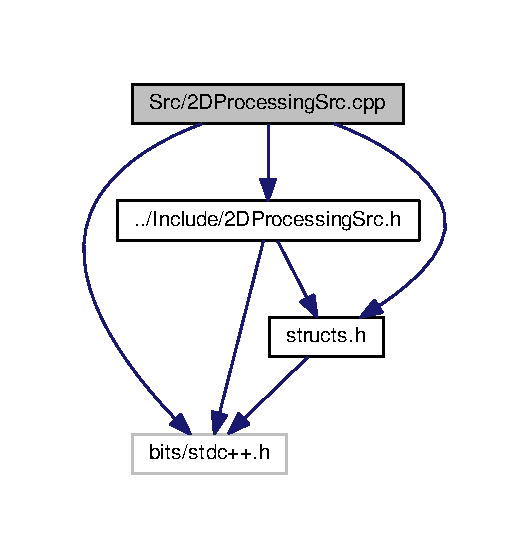
\includegraphics[width=254pt]{2DProcessingSrc_8cpp__incl}
\end{center}
\end{figure}

\hypertarget{3DProcessingSrc_8cpp}{}\section{3\+D\+Processing\+Src.cpp File Reference}
\label{3DProcessingSrc_8cpp}\index{3\+D\+Processing\+Src.\+cpp@{3\+D\+Processing\+Src.\+cpp}}
{\ttfamily \#include $<$bits/stdc++.\+h$>$}\\*
{\ttfamily \#include $<$structs.\+cpp$>$}\\*
Include dependency graph for 3\+D\+Processing\+Src.cpp\+:
% FIG 0
This graph shows which files directly or indirectly include this file\+:
% FIG 1
\subsection*{Classes}
\begin{DoxyCompactItemize}
\item 
class \hyperlink{classThreeDGraph__class}{Three\+D\+Graph\+\_\+class}
\begin{DoxyCompactList}\small\item\em 3D behaviour class. \end{DoxyCompactList}\end{DoxyCompactItemize}

\hypertarget{Graphs_8cpp}{}\section{Graphs.\+cpp File Reference}
\label{Graphs_8cpp}\index{Graphs.\+cpp@{Graphs.\+cpp}}
{\ttfamily \#include $<$bits/stdc++.\+h$>$}\\*
{\ttfamily \#include \char`\"{}2\+D\+Processing\+Src.\+cpp\char`\"{}}\\*
{\ttfamily \#include \char`\"{}3\+D\+Processing\+Src.\+cpp\char`\"{}}\\*
{\ttfamily \#include \char`\"{}structs.\+cpp\char`\"{}}\\*
Include dependency graph for Graphs.\+cpp\+:\nopagebreak
\begin{figure}[H]
\begin{center}
\leavevmode
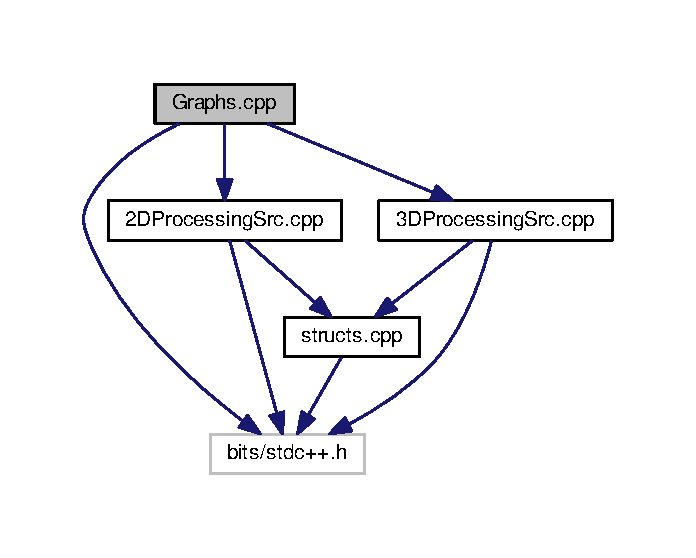
\includegraphics[width=334pt]{Graphs_8cpp__incl}
\end{center}
\end{figure}
This graph shows which files directly or indirectly include this file\+:\nopagebreak
\begin{figure}[H]
\begin{center}
\leavevmode
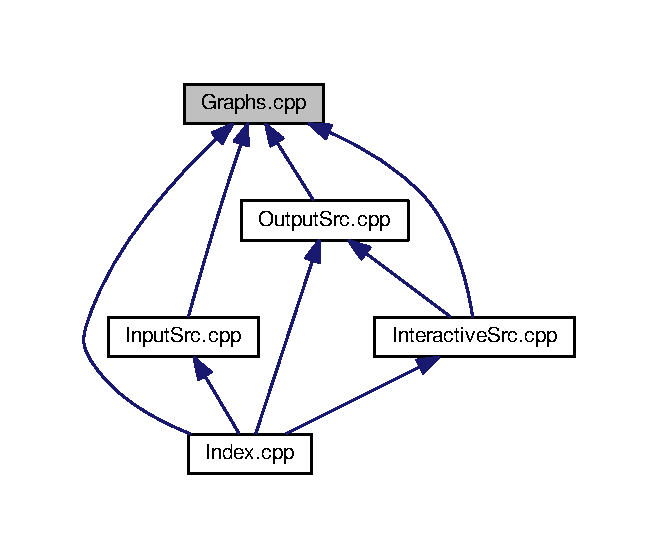
\includegraphics[width=316pt]{Graphs_8cpp__dep__incl}
\end{center}
\end{figure}
\subsection*{Namespaces}
\begin{DoxyCompactItemize}
\item 
 \hyperlink{namespacegraph}{graph}
\begin{DoxyCompactList}\small\item\em Graph namespace. \end{DoxyCompactList}\end{DoxyCompactItemize}
\subsection*{Variables}
\begin{DoxyCompactItemize}
\item 
map$<$ string, vector$<$ \hyperlink{structpoint}{point} $>$ $>$ \hyperlink{namespacegraph_a4315e19997c8b99a403fed5968799e10}{graph\+::\+Three\+D\+Graph}
\item 
map$<$ string, vector$<$ \hyperlink{structpoint}{point} $>$ $>$ \hyperlink{namespacegraph_a18be037bbd2748e849072b9f5017c97e}{graph\+::\+Two\+D\+Graph} \mbox{[}3\mbox{]}
\item 
bool \hyperlink{namespacegraph_aaa8a7bf9ccfc70dd98f403db09e1d57f}{graph\+::\+Three\+D\+Or\+TwoD} = false
\end{DoxyCompactItemize}

\hypertarget{Index_8cpp}{}\section{Index.\+cpp File Reference}
\label{Index_8cpp}\index{Index.\+cpp@{Index.\+cpp}}
{\ttfamily \#include \char`\"{}cop/mainwindow.\+h\char`\"{}}\\*
{\ttfamily \#include $<$Q\+Application$>$}\\*
{\ttfamily \#include \char`\"{}bits/stdc++.\+h\char`\"{}}\\*
{\ttfamily \#include $<$Qt\+Core$>$}\\*
{\ttfamily \#include $<$Qt\+Gui$>$}\\*
{\ttfamily \#include $<$Q\+Label$>$}\\*
{\ttfamily \#include \char`\"{}structs.\+h\char`\"{}}\\*
{\ttfamily \#include \char`\"{}2\+D\+Processing\+Src.\+h\char`\"{}}\\*
{\ttfamily \#include \char`\"{}3\+D\+Processing\+Src.\+h\char`\"{}}\\*
{\ttfamily \#include \char`\"{}Input\+Src.\+h\char`\"{}}\\*
{\ttfamily \#include \char`\"{}Output\+Src.\+h\char`\"{}}\\*
{\ttfamily \#include \char`\"{}Interactive\+Src.\+h\char`\"{}}\\*
{\ttfamily \#include \char`\"{}mainwindow.\+h\char`\"{}}\\*
{\ttfamily \#include \char`\"{}ui\+\_\+mainwindow.\+h\char`\"{}}\\*
{\ttfamily \#include \char`\"{}dialog.\+h\char`\"{}}\\*
{\ttfamily \#include \char`\"{}ui\+\_\+dialog.\+h\char`\"{}}\\*
{\ttfamily \#include \char`\"{}interactiveinput.\+h\char`\"{}}\\*
{\ttfamily \#include \char`\"{}ui\+\_\+interactiveinput.\+h\char`\"{}}\\*
{\ttfamily \#include $<$Q\+File\+Dialog$>$}\\*
{\ttfamily \#include $<$Q\+Dir$>$}\\*
Include dependency graph for Index.\+cpp\+:
% FIG 0
\subsection*{Functions}
\begin{DoxyCompactItemize}
\item 
int \hyperlink{Index_8cpp_a0ddf1224851353fc92bfbff6f499fa97}{main} (int argc, char $\ast$argv\mbox{[}$\,$\mbox{]})
\end{DoxyCompactItemize}
\subsection*{Variables}
\begin{DoxyCompactItemize}
\item 
\hyperlink{classTwoDGraph__class}{Two\+D\+Graph\+\_\+class} {\bfseries input\+\_\+2d}\hypertarget{Index_8cpp_a7b422d961385be1621c787c7778593bb}{}\label{Index_8cpp_a7b422d961385be1621c787c7778593bb}

\item 
\hyperlink{classThreeDGraph__class}{Three\+D\+Graph\+\_\+class} {\bfseries input\+\_\+3d}\hypertarget{Index_8cpp_a594364b5a7f006d761aa9a8cfcb68ea2}{}\label{Index_8cpp_a594364b5a7f006d761aa9a8cfcb68ea2}

\item 
\hyperlink{classInteractive__editor}{Interactive\+\_\+editor} {\bfseries I1}\hypertarget{Index_8cpp_a403922218be213881144c168aac549c3}{}\label{Index_8cpp_a403922218be213881144c168aac549c3}

\item 
\hyperlink{classOutput}{Output} {\bfseries O1}\hypertarget{Index_8cpp_a74c85b6f0cd4748d25b91ba68d28b9be}{}\label{Index_8cpp_a74c85b6f0cd4748d25b91ba68d28b9be}

\item 
\hyperlink{classOutput}{Output} {\bfseries O2}\hypertarget{Index_8cpp_a805ab3302ab876a5f85457d063bf5bbd}{}\label{Index_8cpp_a805ab3302ab876a5f85457d063bf5bbd}

\item 
bool {\bfseries is\+File3d}\hypertarget{Index_8cpp_ab82efbeaa2890f39bf11e2ca4a83ce1b}{}\label{Index_8cpp_ab82efbeaa2890f39bf11e2ca4a83ce1b}

\item 
bool {\bfseries is\+Input\+File}\hypertarget{Index_8cpp_a82277de5e18d1e9caabbdeea50a0cd49}{}\label{Index_8cpp_a82277de5e18d1e9caabbdeea50a0cd49}

\item 
string {\bfseries filename}\hypertarget{Index_8cpp_a3a1a90139c2c8ab1fca0ea8b1790b7b2}{}\label{Index_8cpp_a3a1a90139c2c8ab1fca0ea8b1790b7b2}

\end{DoxyCompactItemize}


\subsection{Function Documentation}
\index{Index.\+cpp@{Index.\+cpp}!main@{main}}
\index{main@{main}!Index.\+cpp@{Index.\+cpp}}
\subsubsection[{\texorpdfstring{main(int argc, char $\ast$argv[])}{main(int argc, char *argv[])}}]{\setlength{\rightskip}{0pt plus 5cm}int main (
\begin{DoxyParamCaption}
\item[{int}]{argc, }
\item[{char $\ast$}]{argv\mbox{[}$\,$\mbox{]}}
\end{DoxyParamCaption}
)}\hypertarget{Index_8cpp_a0ddf1224851353fc92bfbff6f499fa97}{}\label{Index_8cpp_a0ddf1224851353fc92bfbff6f499fa97}
$<$ This is the orthographic projections 
\hypertarget{IndexMayank_8cpp}{}\section{Index\+Mayank.\+cpp File Reference}
\label{IndexMayank_8cpp}\index{Index\+Mayank.\+cpp@{Index\+Mayank.\+cpp}}
{\ttfamily \#include \char`\"{}bits/stdc++.\+h\char`\"{}}\\*
{\ttfamily \#include \char`\"{}Graphs.\+cpp\char`\"{}}\\*
{\ttfamily \#include \char`\"{}Input\+Src.\+cpp\char`\"{}}\\*
{\ttfamily \#include \char`\"{}Output\+Src.\+cpp\char`\"{}}\\*
{\ttfamily \#include \char`\"{}Interactive\+Src.\+cpp\char`\"{}}\\*
Include dependency graph for Index\+Mayank.\+cpp\+:

\hypertarget{InputSrc_8cpp}{}\section{Input\+Src.\+cpp File Reference}
\label{InputSrc_8cpp}\index{Input\+Src.\+cpp@{Input\+Src.\+cpp}}
{\ttfamily \#include $<$bits/stdc++.\+h$>$}\\*
{\ttfamily \#include $<$Input\+Src.\+cpp$>$}\\*
{\ttfamily \#include $<$Output\+Src.\+cpp$>$}\\*
{\ttfamily \#include $<$2\+D\+Processing\+Src.\+cpp$>$}\\*
{\ttfamily \#include $<$3\+D\+Processing\+Src.\+cpp$>$}\\*
{\ttfamily \#include $<$Interactive\+Src.\+cpp$>$}\\*
Include dependency graph for Input\+Src.\+cpp\+:
% FIG 0
This graph shows which files directly or indirectly include this file\+:
% FIG 1
\subsection*{Classes}
\begin{DoxyCompactItemize}
\item 
class \hyperlink{classInput}{Input}
\begin{DoxyCompactList}\small\item\em \hyperlink{classInput}{Input} class. \end{DoxyCompactList}\end{DoxyCompactItemize}

\hypertarget{InteractiveSrc_8cpp}{}\section{Interactive\+Src.\+cpp File Reference}
\label{InteractiveSrc_8cpp}\index{Interactive\+Src.\+cpp@{Interactive\+Src.\+cpp}}
{\ttfamily \#include $<$bits/stdc++.\+h$>$}\\*
{\ttfamily \#include \char`\"{}structs.\+cpp\char`\"{}}\\*
{\ttfamily \#include \char`\"{}Graphs.\+cpp\char`\"{}}\\*
{\ttfamily \#include \char`\"{}Output\+Src.\+cpp\char`\"{}}\\*
{\ttfamily \#include \char`\"{}2\+D\+Processing\+Src.\+cpp\char`\"{}}\\*
{\ttfamily \#include \char`\"{}3\+D\+Processing\+Src.\+cpp\char`\"{}}\\*
Include dependency graph for Interactive\+Src.\+cpp\+:\nopagebreak
\begin{figure}[H]
\begin{center}
\leavevmode
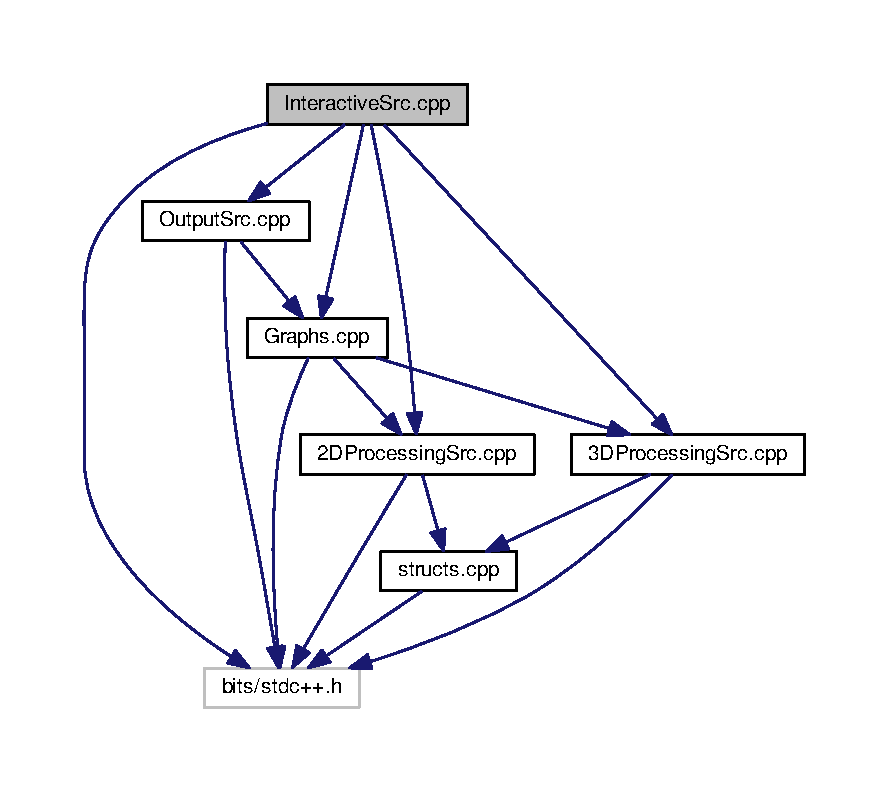
\includegraphics[width=350pt]{InteractiveSrc_8cpp__incl}
\end{center}
\end{figure}
This graph shows which files directly or indirectly include this file\+:\nopagebreak
\begin{figure}[H]
\begin{center}
\leavevmode
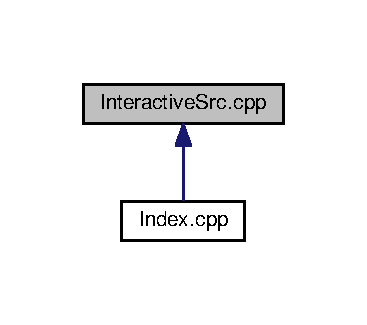
\includegraphics[width=176pt]{InteractiveSrc_8cpp__dep__incl}
\end{center}
\end{figure}
\subsection*{Classes}
\begin{DoxyCompactItemize}
\item 
class \hyperlink{classInteractive__editor}{Interactive\+\_\+editor}
\begin{DoxyCompactList}\small\item\em Editor class. \end{DoxyCompactList}\end{DoxyCompactItemize}

\hypertarget{OutputSrc_8cpp}{}\section{Output\+Src.\+cpp File Reference}
\label{OutputSrc_8cpp}\index{Output\+Src.\+cpp@{Output\+Src.\+cpp}}
{\ttfamily \#include $<$bits/stdc++.\+h$>$}\\*
{\ttfamily \#include $<$Input\+Src.\+cpp$>$}\\*
{\ttfamily \#include $<$Output\+Src.\+cpp$>$}\\*
{\ttfamily \#include $<$2\+D\+Processing\+Src.\+cpp$>$}\\*
{\ttfamily \#include $<$3\+D\+Processing\+Src.\+cpp$>$}\\*
{\ttfamily \#include $<$Interactive\+Src.\+cpp$>$}\\*
Include dependency graph for Output\+Src.\+cpp\+:
% FIG 0
This graph shows which files directly or indirectly include this file\+:
% FIG 1
\subsection*{Classes}
\begin{DoxyCompactItemize}
\item 
class \hyperlink{classOutput}{Output}
\begin{DoxyCompactList}\small\item\em Render and save class. \end{DoxyCompactList}\end{DoxyCompactItemize}

\hypertarget{structs_8cpp}{}\section{structs.\+cpp File Reference}
\label{structs_8cpp}\index{structs.\+cpp@{structs.\+cpp}}
{\ttfamily \#include $<$bits/stdc++.\+h$>$}\\*
Include dependency graph for structs.\+cpp\+:
% FIG 0
This graph shows which files directly or indirectly include this file\+:
% FIG 1
\subsection*{Classes}
\begin{DoxyCompactItemize}
\item 
struct \hyperlink{structpoint}{point}
\begin{DoxyCompactList}\small\item\em Struct point. \end{DoxyCompactList}\item 
struct \hyperlink{structplane}{plane}
\begin{DoxyCompactList}\small\item\em Struct plane. \end{DoxyCompactList}\item 
struct \hyperlink{structedge}{edge}
\begin{DoxyCompactList}\small\item\em Struct edge. \end{DoxyCompactList}\end{DoxyCompactItemize}

%--- End generated contents ---

% Index
\backmatter
\newpage
\phantomsection
\clearemptydoublepage
\addcontentsline{toc}{chapter}{Index}
\printindex

\end{document}
